\chapter{AHTR Modeling and Optimization Methodology}
\glsresetall
\label{chap:method}
In this chapter, I describe the modeling methodology of the 
\gls{AHTR} plank and one-third assembly optimization for non-conventional 
geometries and parameters conducted using the \gls{ROLLO} software.
The optimization tool should enable the placement of fuel, moderator, and coolant 
material in any possible location, within physical limits, to wholly explore the 
design space enabled by additive manufacturing. 
As exploring the design space of non-conventional geometries and parameters on 
reactors has been applied in very limited circumstances (previous attempts described 
in Section \ref{sec:lit-review-reactor-arbitrary}), this dissertation must 
systematically explore and constrain the large design space. 
As this work is a proof of concept, this dissertation is only an intermediate step 
towards developing a truly arbitrary geometry expression. 

The subsequent sections define the optimization problem (Section \ref{sec:opt-problem}), 
describe the \gls{AHTR} geometries (Section \ref{sec:ahtr-geometry}), 
outline the \gls{AHTR} modeling workflow (Section \ref{sec:ahtr-model-workflow}), 
verify the \gls{AHTR} models (Section \ref{sec:ahtr_model_verification}), 
and describe the process of tuning \gls{ROLLO}'s hyperparameters (Section 
\ref{sec:hyperparameter-studies}). 
Appendix A lists all the data and analysis related to this chapter to enable the 
reproduction of all the simulations.

\section{ROLLO Optimization Problem Definitions}
\label{sec:opt-problem}
In an effort toward optimizing the \gls{AHTR} design for non-conventional geometries 
and parameters, 
I chose to vary the following \gls{AHTR} parameters: 
\begin{itemize}
    \item \gls{TRISO} fuel packing fraction distribution ($\rho_{TRISO}(\vec{r})$),
    \item total fuel packing fraction ($PF_{total}$), and 
    \item coolant channel shape.
\end{itemize} 
Varying the \gls{TRISO} fuel packing fraction distribution allows us to explore how 
heterogeneous fuel distributions impact reactor performance.
In Section \ref{sec:fhr-benchmark-keff}, the \gls{FHR} benchmark results demonstrated 
that increased fuel packing does not always correspond with increased $k_{eff}$ due to 
self-shielding effects. 
Varying total fuel packing fraction and TRISO distribution enables synergistic
exploration of how heterogenous TRISO distribution could minimize self-shielding and 
thus, reduce the fuel required for a reactor design. 
The coolant channel shape variation enables exploration of how non-uniform 
channel shapes impacts heat transfer. 

I selected three key \gls{AHTR} optimization objectives that address contrasting reactor 
core qualities. 
Table \ref{tab:objectives} describes each objective, how I quantified them, and the motivation.
\begin{table}[htbp]
    \centering
    \onehalfspacing
    \caption{\acrfull{ROLLO} \acrfull{AHTR} optimization problem objectives with 
    their quantification descriptions and motivation.}
	\label{tab:objectives}
    \footnotesize
    \begin{tabular}{p{4.5cm}|p{5cm}p{5cm}}
    \hline 
    \textbf{Objective}& \textbf{Quantification}& \textbf{Motivation} \\
    \hline
    \textbf{Minimize fuel amount} & Minimize total fuel packing \newline fraction 
    & Cost savings, Non-proliferation \\ 
    \hline
    \textbf{Maximize heat transfer} & Minimize maximum temperature 
    & Minimize thermal stress in the fuel \\
    \hline
    \textbf{Minimize power peaking} & Minimize power peaking factor normalized by fuel distribution 
    & Efficient fuel utilization, longer core life, safety\\
    \hline
    \end{tabular}
\end{table}

To optimize the objectives, I will vary the parameters in the \gls{AHTR} plank and 
one-third assembly models. 
The optimization results for the \gls{AHTR} plank and one-third assembly models are 
reported in Chapters \ref{chap:ahtr-plank-opt-results} and \ref{chap:ahtr-assem-opt-results}, 
respectively. 
The \gls{AHTR} plank optimization is a preliminary study to inform the more complex 
\gls{AHTR} one-third assembly optimization setup. 
In the next section, I will describe both geometries. 

\section{AHTR Geometry for Optimization Problem}
\label{sec:ahtr-geometry}
I apply the optimization process to the \gls{AHTR} plank and \gls{AHTR} one-third
assembly geometries.
The geometries are adapted from the \gls{FHR} benchmark's \gls{AHTR} design,
outlined in Chapter \ref{chap:fhr-benchmark} (see Figure \ref{fig:ahtr-fuel-assembly}).
The main differences occur in the fuel plank region. 
In the \gls{FHR} benchmark, the TRISO particles are arranged in rectangular lattices 
within two fuel stripes in the fuel plank region, shown in Figure 
\ref{fig:ahtr-fuel-plank-2}. 
\begin{figure}[htbp]
    \centering
    \includegraphics[width=0.9\linewidth]{ahtr-fuel-plank.png} 
    \resizebox{0.3\textwidth}{!}{
        \fbox{\begin{tabular}{ll}
            \textcolor{fhrblue}{$\blacksquare$} & FLiBe \\
            \textcolor{fhrgrey}{$\blacksquare$} & Graphite (Fuel Structure)\\
            \textcolor{fhrred}{$\blacksquare$} & Graphite (Fuel Plank) \\
            \textcolor{fhrgreen}{$\blacksquare$} & Graphite (Fuel Stripe) \\
            \textcolor{fhryellow}{$\blacksquare$} & TRISO particle \\
            \textcolor{fhrpink}{$\blacksquare$} & Graphite (Spacer) \\
            \end{tabular}}}
            \hspace{0.5cm}
            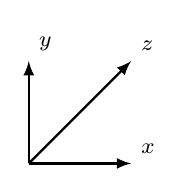
\begin{tikzpicture}
                \draw[ thick,-latex] (0,0) -- (1.3,0) node[anchor=south west] {$x$};
                \draw[ thick,-latex] (0,0) -- (0,1.3) node[anchor=south west] {$y$};
                \draw[ thick,-latex] (0,0) -- (1.3,1.3) node[anchor=south west] {$z$};
               \tkzText[above](-0.5,1){}
               \end{tikzpicture} 
    \caption{\acrfull{FHR} benchmark's \acrfull{AHTR} design's fuel plank, with the 
    magnification of a spacer and segment of the fuel stripe with embedded 
    \gls{TRISO} particles.}
    \label{fig:ahtr-fuel-plank-2}
\end{figure}
For the \gls{AHTR} plank and \gls{AHTR} one-third assembly optimization geometries, 
I discretized each plank into ten cells with random TRISO packing and an individually 
controlled packing fraction. 
Thus, the \gls{AHTR} plank has ten fuel cells, and the \gls{AHTR} one-third assembly 
has 60 fuel cells (10 cells for 6 planks).  
The subsequent subsections describe each geometry in further detail.
I also omit the graphite spacers. 

\subsection{AHTR Plank Geometry}
\label{sec:ahtr-plank-geometry}
The \gls{AHTR} plank is a single graphite fuel plank model from the \gls{AHTR} design 
(Figure \ref{fig:ahtr-fuel-assembly}). 
I modified the fuel plank to be straightened with perpendicular sides instead 
of slanted as in Figure \ref{fig:ahtr-fuel-plank} for ease of modeling. 
The one-third assembly optimization uses the original slanted \gls{AHTR} planks. 
Figure \ref{fig:straightened_plank} illustrates the straightened fuel plank with 
ten fuel cells with random \gls{TRISO} packing in each cell.
\begin{figure}[htbp]
    \centering
    \includegraphics[width=0.85\linewidth]{straightened_plank.png}
    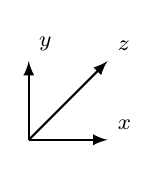
\begin{tikzpicture}
        \draw[ thick,-latex] (0,0) -- (1,0) node[anchor=south west] {$x$};
        \draw[ thick,-latex] (0,0) -- (0,1) node[anchor=south west] {$y$};
        \draw[ thick,-latex] (0,0) -- (1,1) node[anchor=south west] {$z$};
       \tkzText[above](-0.3,-0.7){}
       \end{tikzpicture} 
    \raggedright
    \resizebox{0.4\textwidth}{!}{
        \hspace{1cm}
        \fbox{\begin{tabular}{ll}
            \textcolor{fhrblue}{$\blacksquare$} & \gls{FLiBe} \\
            \textcolor{fhrgrey}{$\blacksquare$} & Graphite (structure)\\
            \textcolor{fhrred}{$\blacksquare$} & Graphite (fuel plank) \\
            \textcolor{fhrblack}{$\blacksquare$} & TRISO particle 

            \end{tabular}}}
    \caption{Straightened \acrfull{AHTR} fuel plank with 10 fuel cells with random 
    TRISO packing, graphite buffers, and straight \gls{FLiBe} coolant channels. 
    This geometry is used for \gls{AHTR} plank optimization.}
    \label{fig:straightened_plank}
\end{figure}
The plank has $27.1 \times 3.25 \times 1.85\ cm^3$ in the x, y, and z dimensions,
respectively, and reflective boundary conditions.

I used the same materials as in the \gls{FHR} benchmark (Chapter \ref{chap:fhr-benchmark}), 
except that I homogenized each \gls{TRISO} particle's four outer layers (porous carbon 
buffer, inner pyrolytic carbon, silicon carbide layer, and the outer pyrolytic carbon) 
into a single layer. 
The \gls{TRISO} kernel and outer radius dimensions remain the same.
Table \ref{tab:keff_triso} reports OpenMC's $k_{eff}$ for the straightened \gls{AHTR} configuration 
with and without the four outer layers \gls{TRISO} homogenization.
\begin{table}[htbp]
    \centering
    \onehalfspacing
    \caption{Straightened \acrfull{AHTR} fuel plank $k_{eff}$ for the case with 
    no \gls{TRISO} homogenization and case with homogenization of the four outer 
    layers. Both simulations were run on one BlueWaters supercomputer XE Node 
    \cite{ncsa_about_2017} using OpenMC \cite{romano_openmc:_2015} with 80 active 
    cycles, 20 inactive cycles, and 8000 particles.}
	\label{tab:keff_triso}
    \footnotesize
    \begin{tabular}{llc}
    \hline 
    \textbf{TRISO Homogenization}& \textbf{$k_{eff}$ [-]} & \textbf{Simulation Time [s]}  \\
    \hline 
    None & $1.38548 \pm 0.00124$ & 233\\ 
    Four outer layers & $1.38625 \pm 0.00109$ & 168\\ 
    \hline
    \end{tabular}
\end{table}
The \gls{TRISO} particle outer four-layer homogenization resulted in a $30\%$ 
speed-up without compromising accuracy with $k_{eff}$ values within each 
other's uncertainty.
As a result, the homogenized models are used for all subsequent optimization efforts. 

\subsection{AHTR One-Third Assembly Geometry}
\label{sec:ahtr-assem-geometry}
The \gls{AHTR} one-third assembly is one-diamond shape sector of the \gls{AHTR} assembly
(Figure \ref{fig:ahtr-fuel-assembly}). 
The one-third assembly contains six graphite fuel planks.
Each graphite fuel plank has graphite buffers and ten rectangular prism fuel cells 
with random TRISO packing and individually controlled packing fractions. 
Figure \ref{fig:ahtr_assembly} shows the one-third \gls{AHTR} assembly with 10 x 6 
fuel cells with random \gls{TRISO} packing.
The one-third assembly model has reflective boundary conditions and  
uses the \gls{TRISO} particle outer four-layer 
homogenization described in Section \ref{sec:ahtr-plank-geometry}.
\begin{figure}[htbp]
    \centering
    \begin{subfigure}{.7\textwidth}
    \includegraphics[width=\linewidth]{ahtr_assembly.png}
    \end{subfigure}%
    \begin{subfigure}{.3\textwidth}
        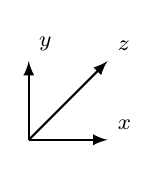
\begin{tikzpicture}
            \draw[ thick,-latex] (0,0) -- (1,0) node[anchor=south west] {$x$};
            \draw[ thick,-latex] (0,0) -- (0,1) node[anchor=south west] {$y$};
            \draw[ thick,-latex] (0,0) -- (1,1) node[anchor=south west] {$z$};
           \tkzText[above](-0.3,-0.7){}
        \end{tikzpicture} 
        \vspace{1cm}
        \fbox{\begin{tabular}{ll}
            \textcolor{fhrblue}{$\blacksquare$} & \gls{FLiBe} \\
            \textcolor{fhrgrey}{$\blacksquare$} & Graphite (structure)\\
            \textcolor{fhrred}{$\blacksquare$} & Graphite (fuel plank) \\
            \textcolor{fhrblack}{$\blacksquare$} & TRISO particle 
            \end{tabular}}
    \end{subfigure}
    \caption{\acrfull{AHTR} one-third assembly with ten randomly packed fuel cells 
    in each graphite plank, graphite structure, and \gls{FLiBe} coolant.}
    \label{fig:ahtr_assembly}
\end{figure}

\section{AHTR Model Workflow}
\label{sec:ahtr-model-workflow}
The \gls{ROLLO} software drives the evolutionary algorithm optimization process, 
depicted in Figure \ref{fig:genetic_alg_nuclear}.
In a \gls{ROLLO} input file, I define control variables that the genetic algorithm 
uses to vary the \gls{AHTR} parameters described in Section \ref{sec:opt-problem}.
The control variables are input into the nuclear software templates to model different 
\gls{AHTR} geometries.
The nuclear software will then run the \gls{AHTR} models and calculate the optimization 
objective and constraint values. 
In this work, I use OpenMC \cite{romano_openmc:_2015} to model \gls{AHTR}'s neutronics 
and Moltres \cite{lindsay_introduction_2018} to model the \gls{AHTR}'s multi-physics. 
Descriptions of each software can be found in Section 
\ref{sec:lit-review-modeling-software}.

In the following subsections, I describe the \gls{AHTR} modeling workflow: the
\gls{AHTR} input parameter variations, the OpenMC and Moltres models, and the output 
and constraint values calculations. 
The \gls{AHTR} modeling workflow described in this section falls within the 
nuclear software evaluation orange blocks in Figure 
\ref{fig:genetic_alg_nuclear}'s genetic algorithm flow chart.
Each \gls{AHTR} modeling workflow models a single reactor model. 
Figure \ref{fig:ahtr-model-flow} illustrates the \gls{AHTR} modeling workflow. 
\begin{figure}[htbp]
    \centering
    \begin{tikzpicture}[node distance=0.5cm]
        \tikzstyle{every node}=[font=\footnotesize]
        %\node (1) [e72block] {\textit{Total PF}};
        \node (2) [g72block] {$PF_{total}$};
        \node (3) [e82block, above=of 2] {Control Variables};
        %\node (4) [e72block, below=of 1] {$\rho_{TRISO}(\vec{r})$};
        \node (5) [g72block, below=of 2] {$\rho_{TRISO}(\vec{r})$};
        %\node (6) [e72block, below=of 4] {\textit{Coolant Channel Shape}};
        \node (7) [g72block, below=of 5] {\textit{Coolant Channel Shape}};
        \node (8) [p72block, right=of 2, xshift=0.8cm, yshift=0.5cm] {OpenMC Model};
        \node (9) [e92block, above=of 8] {Nuclear Software Models};
        \node (10) [p72block, right=of 5, xshift=0.8cm] {Group Constants};
        \node (11) [p72block, right=of 7, xshift=0.8cm, yshift=-0.5cm] {Moltres Model};
        \node (12) [g72block, right=of 8, xshift=0.8cm, yshift=0.8cm] {$k_{eff}$}; 
        \node (13) [e72block, above=of 12] {Constraints};
        \node (14) [e72block, below=of 12] {Objectives};
        \node (15) [g72block, below=of 14] {PF};
        \node (16) [g72block, below=of 15] {$PPF_{fuel}$};
        \node (17) [g72block, below=of 16] {$T_{max}$};
        \draw [arrow] (2) -- ([shift={(0cm,0cm)}]2.east) -- ([shift={(0cm,0cm)}]8.west);
        \draw [arrow] (5) -- ([shift={(0cm,0cm)}]5.east) -- ([shift={(0cm,0cm)}]8.west);
        \draw [arrow] (7) -- ([shift={(0cm,0cm)}]7.east) -- ([shift={(0cm,0cm)}]8.west);
        \draw [arrow] (7) -- ([shift={(0cm,0cm)}]7.east) -- ([shift={(0cm,0cm)}]11.west);
        \draw [arrow] (8) -- ([shift={(0cm,0cm)}]8.south) -- node[anchor=west] {generates} ([shift={(0cm,0cm)}]10.north);
        \draw [arrow] (10) -- ([shift={(0cm,0cm)}]10.south) -- node[anchor=west] {input into} ([shift={(0cm,0cm)}]11.north);
        \draw [arrow] (8) -- ([shift={(0cm,0cm)}]8.east) -- ([shift={(0cm,0cm)}]12.west);
        \draw [arrow] (8) -- ([shift={(0cm,0cm)}]8.east) -- ([shift={(0cm,0cm)}]15.west);
        \draw [arrow] (8) -- ([shift={(0cm,0cm)}]8.east) -- ([shift={(0cm,0cm)}]16.west);
        \draw [arrow] (11) -- ([shift={(0cm,0cm)}]11.east) -- ([shift={(0cm,0cm)}]17.west);
    \end{tikzpicture}
    \caption{\acrfull{AHTR} modeling workflow in \acrfull{ROLLO} optimization.
    For each reactor model in the optimization process, the modeling workflow begins 
    with ROLLO selecting the control variables within the user-defined range. 
    ROLLO inserts control variables and runs the templated OpenMC and Moltres 
    input files. 
    ROLLO analyzes the OpenMC and Moltres output files to determine the constraint and 
    objective values.
    $PF_{total}$: Total fuel packing fraction, $\rho_{TRISO}(\vec{r})$: TRISO packing 
    fraction distribution, $PPF_{fuel}$: normalized power peaking factor, 
    $T_{max}$: model's maximum temperature.} 
    \label{fig:ahtr-model-flow}
\end{figure}

\subsection{Input Parameter Modeling}
\label{sec:input-parameter-modeling}
This subsection describes how I model the \gls{AHTR} input parameter variations: 
total fuel packing fraction ($PF_{total}$), \gls{TRISO} packing fraction distribution
($\rho_{TRISO}(\vec{r})$), and coolant channel shape. 
For both the \gls{AHTR} plank and one-third assembly models, the $PF_{total}$ parameter 
is a single numerical input.
Following this, I describe how I modeled the other two parameters for 
the \gls{AHTR} plank and one-third assembly models. 

\subsubsection{Input Parameter Modeling: TRISO packing fraction distribution 
($\rho_{TRISO}(\vec{r})$)}
I utilize sine distributions for both the \gls{AHTR} plank and one-third assembly 
models to govern the $\rho_{TRISO}(\vec{r})$.
First, I impose an overall sine distribution to represent fuel packing in the model. 
The model calculates each fuel cell's packing fraction based on the midpoint 
x-value of the sine distribution in the cell. 
Then, I use OpenMC's \texttt{pack\_spheres} function to randomly disperse 
the packing fraction in each fuel cell. 
For the \gls{AHTR} plank, one sine distribution governs the $\rho_{TRISO}(\vec{x})$ 
across the \gls{AHTR} plank's x-direction. 
For the \gls{AHTR} one-third assembly, two sine distributions govern the 
$\rho_{TRISO}(\vec{x}, \vec{y})$ across each fuel plank's x-direction and the 
assembly's y-direction, respectively. 

For the \gls{AHTR} plank, the sine distribution that governs the \gls{TRISO} packing 
fraction distribution across the ten fuel cells in the x-direction is given by 
Equation \ref{eq:plank-sine}.
\begin{align}
    \label{eq:plank-sine}
    \rho_{TRISO}(\vec{x}) &= \left(a\cdot sin(b\cdot x + c) + 2\right) \cdot NF\\
    \intertext{where}
    \rho_{TRISO}(\vec{x}) &= \mbox{TRISO packing fraction distribution across ten cells } [-] \nonumber \\ 
    a &= \mbox{amplitude, peak deviation of the function from zero } [-] \nonumber \\
    b &= \mbox{angular frequency, rate of change of the function argument } [radians \cdot cm^{-1}] \nonumber \\
    c &= \mbox{phase, the position in its cycle the oscillation is at t = 0 } [radians]\nonumber \\
    x &= \mbox{midpoint x-value for each cell } [cm]\nonumber \\
    NF &= \mbox{normalization factor } [-]\nonumber
\end{align}
%Appendix A describes the normalization factor's calculation. 
Figure \ref{fig:straightened_plank} depicted the ten fuel cells.
The sine distribution's coefficients, \textit{a b c}, are the control variables 
\gls{ROLLO} utilizes to manipulate the plank's $\rho_{TRISO}(\vec{x})$.
Thus, \gls{ROLLO} will vary the \textit{a, b, c} variables to find an optimal 
$\rho_{TRISO}(\vec{x})$ that optimizes objectives. 
The normalization factor is based on the defined total packing fraction.

An \gls{AHTR} plank with $PF_{total} = 0.0979$, and 
$\rho_{TRISO}(\vec{x}) = \left(0.5\cdot sin(\frac{\pi}{3}\cdot x + \pi) + 2\right) 
\cdot NF$, results in the following packing fractions for the ten cells, respectively: 
0.103, 0.120, 0.049, 0.138, 0.076, 0.081, 0.136, 0.048, 0.125, and 0.098. 
Figure \ref{fig:ahtr-plank-triso-distr} shows this sine distribution, highlights 
the packing fraction at the respective midpoints, and displays the plank's x-y 
axis view with the packing fraction varying based on this sine distribution. 
\begin{figure}[htbp]
    \begin{subfigure}{\textwidth}
        \centering
        \includegraphics[width=0.9\linewidth]{triso_distribution_sine.png}
        \caption{TRISO packing fraction distribution values.}
        \label{fig:ahtr-plank-triso-distr-squares} 
    \end{subfigure}
    \begin{subfigure}{\textwidth}
        \centering
        \includegraphics[width=\linewidth]{triso_distribution_plank.png}
        \raggedright
        \resizebox{0.3\textwidth}{!}{
        \hspace{1cm}
        \fbox{\begin{tabular}{ll}
            \textcolor{fhrblue}{$\blacksquare$} & \gls{FLiBe} \\
            \textcolor{fhrgrey}{$\blacksquare$} & Graphite (structure) \\
            \textcolor{fhrred}{$\blacksquare$} & Graphite (fuel plank) \\
            \textcolor{fhrblack}{$\blacksquare$} & TRISO particle 
        \end{tabular}}}
        \caption{TRISO distribution in plank model.}
        \label{fig:ahtr-plank-triso-distr} 
    \end{subfigure}
    \caption{Straightened \acrfull{AHTR} fuel plank with varying \gls{TRISO} particle 
        distribution across 10 cells based on the sine distribution: 
        $\rho_{TRISO}(\vec{x}) = (0.5\ sin(\frac{\pi}{3}x + \pi) + 2)  \times NF$.
        Figure \ref{fig:ahtr-plank-triso-distr-squares}'s packing fraction values 
        correspond to Figure \ref{fig:ahtr-plank-triso-distr}'s  TRISO distribution in 
        the plank model.}
\end{figure}

For the \gls{AHTR} one-third assembly, Equation \ref{assem-sine}'s two sine 
distributions govern \gls{TRISO} packing fraction distributions in the x and y direction 
for the 10 x 6 fuel cells:
\begin{align}
    \label{assem-sine}
    \rho_{TRISO}(\vec{x}, \vec{y}) &= \left(a\cdot sin(b\cdot x + c) + 2\right) 
    \cdot \left(d\cdot sin(e\cdot y + f) + 2\right) \cdot NF \\
    \intertext{where}
    \rho_{TRISO}(\vec{x}, \vec{y}) &= \mbox{TRISO packing fraction distribution across 60 cells } [-] \nonumber \\ 
    a, d &= \mbox{amplitude, peak deviation of the function from zero } [-] \nonumber \\
    b, e &= \mbox{angular frequency, rate of change of the function argument } [radians \cdot cm^{-1}] \nonumber \\
    c, f &= \mbox{phase, the position in its cycle the oscillation is at t = 0 } [radians]\nonumber \\
    x &= \mbox{midpoint value for each x-direction fuel cell } [cm]\nonumber \\
    y &= \mbox{midpoint value for each fuel plank } [cm]\nonumber \\
    NF &= \mbox{normalization factor } [-]\nonumber
\end{align}
Figure \ref{fig:ahtr_assembly} depicts the 10 x 6 fuel cells.
The sine distribution's coefficients, \textit{a b c d e f}, are the control variables 
\gls{ROLLO} utilizes to manipulate the $\rho_{TRISO}(\vec{x}, \vec{y})$ in the 
one-third assembly.
Thus, \gls{ROLLO} will vary \textit{a b c d e f} constants to find an optimal 
$\rho_{TRISO}(\vec{x}, \vec{y})$ that optimizes objectives.
The normalization factor is based on the defined total packing fraction.

An \gls{AHTR} one-third assembly with $PF_{total} = 0.1$ and 
$\rho_{TRISO}(\vec{x}, \vec{y}) = \left(0.5\cdot sin(1\cdot x + 1) + 2\right) \cdot 
\left(0.7\cdot sin(1.5\cdot y + 2) + 2\right) \cdot NF$ results in the packing fraction 
distribution shown in Figure \ref{fig:ahtr-assem-triso-distr-squares}, which 
corresponds to the one-third assembly with varying TRISO distribution in its fuel 
cells, shown in Figure \ref{fig:ahtr-assem-triso-distr}. 
\begin{figure}[htbp]
    \begin{subfigure}{0.49\textwidth}
        \centering
        \includegraphics[width=\linewidth]{ahtr-assem-triso-distr-squares.png}
        \caption{TRISO packing fraction distribution values.}
        \label{fig:ahtr-assem-triso-distr-squares} 
    \end{subfigure}
    \begin{subfigure}{0.49\textwidth}
        \centering
        \includegraphics[width=\linewidth]{ahtr-assem-triso-distr.png}
        \raggedleft
        \resizebox{0.5\textwidth}{!}{
        \hspace{1cm}
        \fbox{\begin{tabular}{ll}
            \textcolor{fhrblue}{$\blacksquare$} & \gls{FLiBe} \\
            \textcolor{fhrgrey}{$\blacksquare$} & Graphite (structure) \\
            \textcolor{fhrred}{$\blacksquare$} & Graphite (fuel plank) \\
            \textcolor{fhrblack}{$\blacksquare$} & TRISO particle 
        \end{tabular}}}
        \caption{TRISO distribution in one-third assembly model.}
        \label{fig:ahtr-assem-triso-distr} 
    \end{subfigure}
    \caption{\acrfull{AHTR} one-third assembly with varying \gls{TRISO} particle 
        distribution across 10 x 6 cells based on the sine distributions: 
        $\rho_{TRISO}(\vec{x}, \vec{y}) = 
        \left(0.5\cdot sin(1\cdot x + 1) + 2\right) \cdot 
        \left(0.7\cdot sin(1.5\cdot y + 2) + 2\right) \cdot NF$. 
        Figure \ref{fig:ahtr-assem-triso-distr-squares}'s packing fraction values 
        correspond to Figure \ref{fig:ahtr-assem-triso-distr}'s  TRISO distribution in 
        the one-third assembly model.}
\end{figure}

\subsubsection{Input Parameter Modeling: Coolant Channel Shape}
For both the \gls{AHTR} plank and one-third assembly models, I simulate the variation in 
coolant channel shape with a sinusoidal pattern using OpenMC's cylinder surfaces
functionality.
By varying the cylinders' radii, the coolant channel shapes' depth and frequency 
mimic a sinusoidal pattern.
I vary the \gls{FLiBe} coolant channel shape while holding the total coolant volume 
constant. 
Holding the coolant volume constant throughout the coolant channel 
optimization process enables the use of the same heat transfer coefficient ($h$)
for all the \gls{AHTR} Moltres temperature models of varying coolant channel shapes.  

For the \gls{AHTR} plank, the $r_{top}$ and $r_{bot}$ variables control the coolant channel 
shape on the top and bottom \gls{FLiBe} channels. 
Figure \ref{fig:coolant-channel-shape} shows the \gls{AHTR} plank's coolant channel 
shape for $r_{top} = 0.2$ and $r_{bot} = 0.3$.
\begin{figure}[htbp]
    \centering
        \includegraphics[width=\linewidth]{coolant-channel-shape.png}
    \raggedright
    \resizebox{0.3\textwidth}{!}{
        \hspace{1cm}
        \fbox{\begin{tabular}{ll}
            \textcolor{fhrblue}{$\blacksquare$} & \gls{FLiBe} Coolant\\
            \textcolor{fhrgrey}{$\blacksquare$} & Graphite (structure) \\
            \textcolor{fhrred}{$\blacksquare$} & Graphite (fuel plank) \\
            \textcolor{fhrblack}{$\blacksquare$} & TRISO particle 
        \end{tabular}}}
    \caption{\acrfull{AHTR} plank with coolant channel shape variation, $r_{top} 
    = 0.2cm$ and $r_{bot} = 0.3cm$.}  
    \label{fig:coolant-channel-shape}
\end{figure}
Thus, \gls{ROLLO} will vary $r_{top}$ and $r_{bot}$ to find optimal coolant 
channel shapes that optimizes objectives.

For the \gls{AHTR} one-third assembly, $r_1, r_2, r_3, r_4, r_5$ variables control the
coolant channel shape in the inter-plank \gls{FLiBe}. 
Figure \ref{fig:coolant-channel-shape-assem} shows the \gls{AHTR} one-third assembly's 
inter-plank coolant channel shapes for $r_1, r_2, r_3, r_4, r_5 = 0.3, 0.2, 0.1, 0.2, 0.3$.
\begin{figure}[htbp]
    \centering
    \begin{subfigure}{.8\textwidth}
    \includegraphics[width=\linewidth]{coolant-channel-shape-assem.png}
    \end{subfigure}%
    \begin{subfigure}{.2\textwidth}
        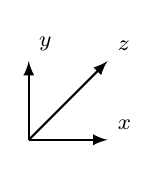
\begin{tikzpicture}
            \draw[ thick,-latex] (0,0) -- (1,0) node[anchor=south west] {$x$};
            \draw[ thick,-latex] (0,0) -- (0,1) node[anchor=south west] {$y$};
            \draw[ thick,-latex] (0,0) -- (1,1) node[anchor=south west] {$z$};
           \tkzText[above](-0.3,-0.7){}
        \end{tikzpicture} 
        \vspace{1cm}
        \resizebox{1.2\textwidth}{!}{
        \fbox{\begin{tabular}{ll}
            \textcolor{fhrblue}{$\blacksquare$} & \gls{FLiBe} \\
            \textcolor{fhrgrey}{$\blacksquare$} & Graphite (structure)\\
            \textcolor{fhrred}{$\blacksquare$} & Graphite (fuel plank) \\
            \textcolor{fhrblack}{$\blacksquare$} & TRISO particle 
            \end{tabular}}}
    \end{subfigure}
    \caption{\acrfull{AHTR} one-third assembly with coolant channel shape variation, 
    $r_1, r_2, r_3, r_4, r_5 = 0.3cm, 0.2cm, 0.1cm, 0.2cm, 0.3cm$.}
    \label{fig:coolant-channel-shape-assem}
\end{figure}
Thus, \gls{ROLLO} will vary $r_1, r_2, r_3, r_4, r_5$ to find optimal coolant 
channel shapes for the \gls{AHTR} one-third assembly model.
I did not vary the shape of the one-third assembly's top and bottom coolant channels, 
since they have half the thickness of the inner coolant channels.  
$r_1, r_2, r_3, r_4, r_5$ are sufficient to show the effect of changing the 
coolant channel shape.

\subsection{AHTR OpenMC and Moltres Models}
\label{sec:ahtr-moltres-hom}
The input parameters outlined in the previous section are inputs for 
the OpenMC neutronics and Moltres temperature models. 
The Moltres model relies on group constant data produced by the OpenMC model. 
The OpenMC and Moltres models' workflow are: 
\begin{enumerate}
\item Run transport with OpenMC neutronics model to calculate $k_{eff}$ and 
fuel-normalized power peaking factor ($PPF_{fuel}$) objective value
\item Produce group constant data for the Moltres model with the OpenMC neutronics model
\item Generate mesh for Moltres model
\item Run Moltres temperature model (accepts group constant data and mesh) to calculate 
maximum temperature ($T_{max}$) objective value
\end{enumerate}
In the subsequent subsections, I describe details and assumptions for each step of 
the OpenMC and Moltres models' workflow.

\subsubsection{AHTR OpenMC Neutronics Model}
The OpenMC model template generates an \gls{AHTR} model from the following \gls{ROLLO} 
input parameters: 
total fuel packing fraction ($PF_{total}$), TRISO distribution ($a, b, c, d, e, f$), 
and coolant channel shapes ($r_{top}, r_{bot}, r_1, r_2, r_3, r_4, r_5$).
\gls{ROLLO} takes these input parameters and generates an OpenMC AHTR model with 
TRISO distribution and FliBe coolant channel shape variation. 
The OpenMC simulations are run with 80 active cycles, 20 inactive cycles, and 8000 
particles resulting in an uncertainty between $\sim 100-150 pcm$.
After the transport simulation is complete, a separate OpenMC file analyzes 
the OpenMC model's output files and calculates the $k_{eff}$ constraint and the 
normalized power peaking factor ($PPF{fuel}$) objective value.
Section \ref{sec:ahtr_slab_output} describes the calculation for each output and 
constraint value.

\subsubsection{AHTR Moltres Group Constant Generation}
\label{sec:ahtr-moltres-group-constant-gen}
Unlike the OpenMC model, Moltres does not explicitly model each \gls{TRISO}
particle. 
This is because a TRISO-level fidelity mesh file is impractical for this simulation 
and results in intractable runtimes. 
Instead, Moltres relies on the OpenMC model to generate group constant data for the 
Moltres' multigroup neutron diffusion calculations. 
Previously, Moltres could only generate group constant data from Serpent 
\cite{leppanen_serpent_2014} or SCALE \cite{bucholz_scale:_1982} output files. 
I implemented functionality in Moltres for group constant data generation with 
OpenMC \cite{lindsay_moltres_2017}. 

To enable successful Moltres \gls{AHTR} temperature model simulations, I must 
establish suitable spatial and energy homogenization for group constant generation. 
These homogenizations must preserve accuracy while maintaining an acceptable runtime.
I compared the key neutronics parameters ($k_{eff}$, reactivity coefficients, 
flux distribution, neutron energy spectrum) for the continuous OpenMC and multigroup 
Moltres simulations (that utilized OpenMC generated group constants) for both the 
\gls{AHTR} plank and one-third assembly to ensure that the selected spatial and energy 
homogenizations preserve accuracy.
Section \ref{sec:ahtr_model_verification} reports the verification study's results.
Next, I describe the energy and spatial homogenizations used. 

For both the \gls{AHTR} plank and one-third assembly models, I used eight precursor 
groups and a 4-group energy structure derived by Gentry et al. 
\cite{gentry_development_2016} for \gls{AHTR} geometries. 
Table \ref{tab:energy_structures} defines the 4-group energy boundaries. 
\begin{table}[htbp]
    \centering
    \onehalfspacing
    \caption{4-group energy structures for \acrfull{AHTR} geometry 
    derived by Gentry et al. \cite{gentry_development_2016}.}
	\label{tab:energy_structures}
    \footnotesize
    \begin{tabular}{lll}
    \hline
    \multicolumn{3}{c}{\textbf{Group Boundaries [MeV]}} \\ 
    \hline
    \textbf{Group $\#$}& \textbf{Upper Bound} & \textbf{Lower Bound}  \\
    \hline 
    1 & $2.0000\times 10^1$ & $9.1188\times 10^{-3}$ \\ 
    2 & $9.1188\times 10^{-3}$ & $2.9023\times 10^{-5}$\\
    3 & $2.9023\times 10^{-5}$ & $1.8554\times 10^{-6}$\\
    4 & $1.8554\times 10^{-6}$ & $1.0000\times 10^{-12}$\\
    \hline
    \end{tabular}
\end{table}

For spatial homogenization of the straightened \gls{AHTR} plank and 
one-third assembly, I used OpenMC's cell domain type to compute 
multigroup cross sections for different cells. 
For the \gls{AHTR} plank, I discretized the plank into 13 cells:
FLiBe, left graphite, right graphite, and ten fuel cells (where each cell has a 
different packing fraction and thus a different material definition).
Figure \ref{fig:straightened_slab_mg} illustrates the \gls{AHTR} plank's spatial 
homogenization for the OpenMC multigroup calculation for Moltres group constant 
generation. 
\begin{figure}[htbp]
    \centering
    \includegraphics[width=\linewidth]{straightened_slab_mg.png}
    \raggedright
    \resizebox{0.5\textwidth}{!}{
        \hspace{1cm}
        \fbox{\begin{tabular}{llll}
            \textcolor{fhrblue}{$\blacksquare$} & \gls{FLiBe} & 
            \textcolor{fhrgrey}{$\blacksquare$} & Left Graphite \\
            \textcolor{fhrred}{$\blacksquare$} & Right Graphite &
            \textcolor{fhrpink}{$\blacksquare$} & Fuel cell 1/6 \\
            \textcolor{fhryellow}{$\blacksquare$} & Fuel cell 2/7 &
            \textcolor{fhrorange}{$\blacksquare$} & Fuel cell 3/8 \\
            \textcolor{fhrgreen}{$\blacksquare$} & Fuel cell 4/9 &
            \textcolor{fhrpurple}{$\blacksquare$} & Fuel cell 5/10 \\
            \end{tabular}}}
    \caption{Straightened \acrfull{AHTR} fuel plank spatially discretized into 
    13 \textit{cells} for OpenMC multigroup calculation to produce group constants 
    data for the Moltres model. 13 \textit{cells}:
    FLiBe, left graphite, right graphite, and ten fuel cells (each cell has a different 
    packing fraction).}
    \label{fig:straightened_slab_mg}
\end{figure}

For the \gls{AHTR} one-third assembly, I discretized the one-third assembly into 
70 \textit{cells}: inter-assembly \gls{FLiBe}, Y-shaped graphite structure, control 
rod slot \gls{FLiBe}, inter-plank \gls{FLiBe}, each graphite plank (6), and ten fuel 
cells per plank (60).
Figure \ref{fig:fhr_onethird_assem_homogenization} illustrates the \gls{AHTR} 
one-third assembly's spatial homogenization for the OpenMC multigroup calculation
for group constant generation. 
\begin{figure}[htbp]
    \centering
    \includegraphics[width=\linewidth]{fhr_onethird_assem_homogenization.png}
    \raggedright
    \resizebox{0.5\textwidth}{!}{
        \hspace{1cm}
        \fbox{\begin{tabular}{ll}
            \textcolor{fhrblue1}{$\blacksquare$} & Inter-assembly \gls{FLiBe} \\
            \textcolor{fhrgrey1}{$\blacksquare$} & Y-shaped graphite structure \\
            \textcolor{fhrblue2}{$\blacksquare$} & Control rod slot \gls{FLiBe} \\
            \textcolor{fhrblue3}{$\blacksquare$} & Inter-plank \gls{FLiBe} \\
            \textcolor{fhrred1}{$\blacksquare$} & Graphite planks \\
            \textcolor{fhrblack1}{$\blacksquare$} \textcolor{fhrwhite1}{$\blacksquare$} & fuel cells
            \end{tabular}}}
    \caption{\acrfull{AHTR} one-third assembly spatially discretized into 
    70 \textit{cells} for OpenMC multigroup calculation to produce group constants 
    data for Moltres model.
    70 \textit{cells}: inter-assembly \gls{FLiBe}, Y-shaped graphite structure, control 
    rod slot \gls{FLiBe}, inter-plank \gls{FLiBe}, each graphite plank (6), and ten fuel 
    cells per plank (60).}
    \label{fig:fhr_onethird_assem_homogenization}
\end{figure}

\subsubsection{AHTR Moltres Mesh Generation}
I wrote Python scripts for the \gls{AHTR} plank and one-third assembly models 
that accept the coolant channel shape input parameters 
($r_{top}, r_{bot}, r_1, r_2, r_3, r_4, r_5$) to generate a geometry script file 
(\texttt{.geo}) based on the spatial homogenizations outlined in the previous 
subsection.
The \gls{AHTR} geometry mesh is then generated from the geometry script file using 
Gmsh \cite{geuzaine_gmsh_2009}.
I used Gmsh's \textit{refine by splitting} functionality to refine the mesh. 
Figures \ref{fig:ahtr-plank-geo} and \ref{fig:ahtr-assem-geo} show Gmsh rendered 
geometry file examples generated by the geometry scripts for the \gls{AHTR} plank 
and one-third assembly, respectively.
\begin{figure}[htbp]
    \centering
    \begin{subfigure}{\textwidth}
        \includegraphics[width=\linewidth]{ahtr-plank-geo.png}
        \caption{\acrfull{AHTR} plank geometry file}
        \label{fig:ahtr-plank-geo} 
    \end{subfigure}
    \begin{subfigure}{\textwidth}
        \includegraphics[width=\linewidth]{ahtr-assem-geo.png}
        \caption{\acrfull{AHTR} one-third assembly geometry file}
        \label{fig:ahtr-assem-geo} 
    \end{subfigure}
    \caption{Examples of \gls{AHTR} plank (Figure \ref{fig:ahtr-plank-geo}) and 
    one-third assembly (Figure \ref{fig:ahtr-assem-geo}) Gmsh rendered geometry files 
    generated by the geometry scripts.
    These geometry files are meshed using Gmsh, and the mesh files are used in the 
    Moltres temperature models.}
\end{figure}

\subsubsection{AHTR Moltres Temperature Model}
\label{sec:ahtr-moltres-temperature-model}
The Moltres \gls{AHTR} steady-state temperature models are a 2D x-y cross-section 
model of the \gls{AHTR} plank and one-third assembly.
The plank and one-third assembly spatially homogenized geometries are depicted in
Figure \ref{fig:straightened_slab_mg} and Figure 
\ref{fig:fhr_onethird_assem_homogenization}.  
Both Moltres temperature models first solve the \gls{AHTR} neutronics and use the 
outputs to solve the \gls{AHTR}'s temperature distribution for a defined power.
The temperature models assume conductive heat transfer throughout the domain 
and heat removal by uniform salt flow in the coolant region. 
These assumptions ignore turbulent effects that would most likely be present. 
However, in-depth \gls{AHTR} Moltres models that includes turbulence modeling is 
a fruitful avenue for future work beyond this dissertation. 

Moltres solves the 4-group diffusion equations 
(Equation \ref{eq:moltres-diffusion-equation}) 
as a steady-state eigenvalue problem to find $k_{eff}$ for the static \gls{AHTR} models.
In the 2D cross-sectional \gls{AHTR} steady-state temperature models, I ignore the 
time-dependent and velocity-dependent terms from Moltres' temperature governing 
equation, shown in Equation \ref{eq:moltres-temp-2}, as they are steady-state models 
with no moving fuel, resulting in Equation \ref{eq:moltres-temp-ss}. 
\begin{align}
    \label{eq:moltres-temp-2}
    \rho c_{p} \frac{\partial T}{\partial t} &= - \rho c_p \vec{u}
    \cdot \nabla T + \nabla \cdot \left(k_i \nabla T \right) + Q_f \\
    \label{eq:moltres-temp-ss}
    - \nabla \cdot (k_i \nabla T) &= Q_i
\intertext{where}
k_i &= \mbox{thermal conductivity of material i } [Wcm^{-1}K^{-1}] \nonumber \\
T &= \mbox{temperature in the model } [K] \nonumber \\
Q_i &= \mbox{source or sink term in material i } [W cm^{-2}] \nonumber
\end{align} 
I use insulated temperature boundary conditions, which mimics an insulator at the 
boundary.
Table \ref{tab:ahtr-thermal-conductivity} shows the thermal conductivity values 
used for each \gls{AHTR} material. 
\begin{table}[htbp]
    \centering
    \onehalfspacing
    \caption{\acrfull{AHTR} materials' thermal conductivities used in Moltres 
    temperature models, taken from \cite{ramey_methodology_2021}.}
	\label{tab:ahtr-thermal-conductivity}
    \footnotesize
    \begin{tabular}{lc}
    \hline 
    \textbf{Material}& \textbf{Thermal Conductivity} \\
    & [$Wcm^{-1}K^{-1}$] \\ 
    \hline 
    \gls{FLiBe} & 0.01 \\
    Graphite  & 0.15 \\
    Fuel  & 0.099 \\
    \hline
    \end{tabular}
\end{table}

Equation \ref{eq:moltres-source-term} defines the fuel cells' fission source term 
($Q_f$):
\begin{align}
\label{eq:moltres-source-term}
    Q_f &= \sum_{g=1}^G \epsilon_{f,g}\Sigma_{f,g}\phi_g
\intertext{where} 
Q_f &= \mbox{source term } [Wcm^{-3}] \nonumber \\
G &= \mbox{number of discrete groups, g } [-] \nonumber \\
\epsilon_{f,g} &= \mbox{heat produced per fission in group g} [J] \nonumber \\
\Sigma_{f,g} &= \mbox{macroscopic cross section for fission due to neutrons in group g } [cm^{-1}] \nonumber \\
\phi_g &= \mbox{flux of neutrons in group g } [n \cdot cm^{-2} s^{-1}]\nonumber
\end{align}

Equation \ref{eq:moltres-heat-removal} defines the heat removal from the \gls{AHTR} 
models:
\begin{align}
    \label{eq:moltres-heat-removal}
    Q &= h \cdot A \cdot(T(\vec{r})-T_{ref})
\intertext{where}
Q &= \mbox{heat removal rate for 1cm thin slice of the AHTR model } [W] \nonumber \\
h &= \mbox{heat transfer coefficient } [W cm^{-2} K^{-1}] \nonumber \\
A &= \mbox{coolant area } [cm^2] \nonumber \\
T(r) &= \mbox{temperature at point r [K]} \nonumber \\
T_{ref} &= \mbox{reference temperature [K]} \nonumber
\end{align}

Table \ref{tab:heat-exchanger-constants} shows reference temperature and heat 
transfer coefficient values for the convective heat transfer process.
\begin{table}[htbp]
    \centering
    \onehalfspacing
    \caption{\acrfull{AHTR} plank and one-third assembly heat transfer constants.}
	\label{tab:heat-exchanger-constants}
    \footnotesize
    \begin{tabular}{lllll}
    \hline 
    \textbf{Model} & \textbf{Constant}& \textbf{Value}& \textbf{Units} & \textbf{Notes} \\
    \hline 
    Plank & $h_{plank}$ & 990 & $W cm^{-2} K^{-1}$ & Calculated in Eq. \ref{eq:calc-htc-plank} \\
    One-Third Assembly & $h_{assem}$ & 611 & $W cm^{-2} K^{-1}$ & Calculated in Eq. \ref{eq:calc-htc-assem} \\
    Both & $T_{ref}$ & 923 & K & AHTR Inlet Temperature \cite{ramey_methodology_2021} \\ 
    \hline
    \end{tabular}
\end{table} 

I calculated the heat transfer coefficient ($h$) for the \gls{AHTR} plank and one-third 
assembly using Equation \ref{eq:calc-htc-plank}, \ref{eq:calc-htc-assem} with the 
following assumptions: 
\begin{itemize}
    \item the \gls{AHTR} modeled generates a constant amount of power, which is all 
    removed by the coolant
    \item a linear increase in temperature from inlet to outlet 
\end{itemize}
\begin{align}
\intertext{The linear temperature change is given by:}
    \Delta T  &= \frac{T_{total}}{H} = \frac{50\ K}{550\ cm} \times 1cm = 0.0909\ K
\intertext{For the plank, $h$ is calculated by: }
    \label{eq:calc-htc-plank}
    h_{plank} &= \frac{P_{dz}}{V_{coolant} \cdot \Delta T} \\
      &= \frac{1456\ W}{(23.1\ cm \times 0.35\ cm \times 2) \cdot 0.0909\ K} \nonumber \\
      &= 990\ W cm^{-2}K^{-1} \nonumber \\
\intertext{and for the one-third assembly: }
      \label{eq:calc-htc-assem}
      h_{assem} &= \frac{P_{dz}}{V_{coolant} \cdot \Delta T} \\
      &= \frac{8741\ W}{157\ cm^2 \cdot 0.0909\ K} \nonumber \\
      &= 611\ W cm^{-1}K^{-1} \nonumber 
\intertext{The relevant parameters for each equation are: }
h_{plank} &= \mbox{plank's heat transfer coefficient } [W cm^{-2} K^{-1}] \nonumber \\
h_{assem} &= \mbox{one-third assembly's heat transfer coefficient } [W cm^{-2} K^{-1}] \nonumber \\
P_{dz} &= \mbox{power produced in 1cm AHTR plank/one-third assem $\Delta z$ slice } [W] \nonumber \\
A_{coolant} &= \mbox{coolant area in AHTR plank/one-third assem } [cm^2] \nonumber \\
\Delta T &= \mbox{temperature change across 1cm AHTR $\Delta z$ slice } [K] \nonumber \\
T_{total} &= \mbox{total temperature change from inlet to outlet } [K] \nonumber \\
H &= \mbox{AHTR height from inlet to outlet } [cm] \nonumber 
\end{align}
The power produced by the \gls{AHTR} plank and one-third models are calculated based 
on the \gls{FHR} benchmark model's specific power of 200 $W gU^{-1}$ and the FHR 
benchmark's TRISO packing fractions in the plank and one-third assembly.
During the optimization simulations in which I vary the $PF_{total}$, I assume that power 
remains constant. 

In the \gls{ROLLO} optimization simulations, I vary the \gls{FLiBe} coolant channel 
shape. 
During the coolant channel shape variation, I hold the coolant volume constant. 
Since the coolant volume is held constant throughout the coolant channel 
optimization process, I use the same heat transfer coefficient ($h$)
for all the \gls{AHTR} Moltres temperature models of varying coolant channel shapes.  

\subsection{Output Parameter Calculation}
\label{sec:ahtr_slab_output}
This section describes how I tallied the \gls{AHTR} model outputs for the ROLLO 
optimization problem objectives (described in Table \ref{tab:objectives}); that is, 
the total fuel packing fraction ($PF_{total}$), the maximum temperature ($T_{max}$), and 
the fuel-normalized power peaking factor ($PPF_{fuel}$).  

\gls{ROLLO} will automatically return the $PF_{total}$ output parameter 
since it is also an input parameter.  
In the Moltres \gls{AHTR} model, I defined a post processor object to return $T_{max}$. 
The $PPF_{fuel}$ output parameter takes into account fuel density variations across 
the model.
For the \gls{AHTR} plank, and each fuel plank in the \gls{AHTR} one-third fuel assembly, 
I discretized the fuel cell area of the plank into 10 $\times$ 5 blocks.
I then use OpenMC to tally the fission energy production rate 
(\texttt{fission-q-recoverable}) in each section. 
\texttt{fission-q-recoverable}'s units are eV per source particle.
Because the final $PPF_{fuel}$ is a ratio, I did not normalize the score to calculate 
power.
The fuel-normalized power peaking factor is given by Equation \ref{eq:ppf}: 
\begin{align}
    \label{eq:ppf}
    PPF_{fuel} &= max(\frac{fqr_j}{PF_j}) \div avg(\frac{fqr_j}{PF_j})
\intertext{where}
PPF_{fuel} &= \mbox{fuel-normalized power peaking factor } [-] \nonumber \\
j &= \mbox{discretized fuel area j } [-] \nonumber \\
fqr_j &= \mbox{fission-q-recoverable at position j } [eV src^{-1}] \nonumber \\
PF_j &= \mbox{fuel packing fraction at position j } [-] \nonumber
\end{align}

\section{AHTR Moltres Model Verification}
\label{sec:ahtr_model_verification}
This section verifies Moltres' ability to reproduce key neutronics parameters 
using group constant data from OpenMC, which is essential for accurate neutronics 
calculations in the Moltres temperature models.
I set up a criticality eigenvalue problem in Moltres and calculate key neutronics 
parameters using group constant data from OpenMC. 
For both the \gls{AHTR} plank and one-third assembly models, I compare the key neutronics 
parameters between two simulations:
\begin{enumerate}
    \item OpenMC simulation with continuous energy and TRISO-level spatial fidelity 
    \item Moltres simulation with 4-group energy and spatial homogenization
\end{enumerate}
Section \ref{sec:ahtr-moltres-group-constant-gen} outlined the spatial homogenization used.
The OpenMC simulation with TRISO-level fidelity generates the group constants for the 
energy and spatially homogenized Moltres simulation. 

I compare the following key neutronics parameters for both the \gls{AHTR} plank 
and one-third assembly models: effective multiplication factor, reactivity coefficients, 
flux distribution, and neutron energy spectrum.  
The comparisons are to verify that the Moltres model is replicating the OpenMC 
model's neutronics correctly.
And of these, comparisons of the reactivity coefficients and flux distributions 
are key to ensuring that Moltres accurately calculates the \gls{AHTR}'s 
temperature distribution.
The reactivity coefficients capture temperature reactivity feedback on the flux 
when the temperature varies with space in the Moltres model. 
The heat produced per fission, $\epsilon_{f,g}$, and macroscopic cross section 
for fission, $\Sigma_{f,g}$, terms in the Moltres source term (Equation 
\ref{eq:moltres-source-term}) are provided to Moltres through 
the group constants generated by the transport software, OpenMC.
Thus, differences in the source term between OpenMC and Moltres are dependent on 
the flux. 

\subsection{AHTR Plank: Key Neutronics Parameters Verification}
\label{sec:plank-knp}
I compare the following key neutronics parameters: effective 
multiplication factor, reactivity coefficients, flux distribution, and neutron energy 
spectrum for the \gls{AHTR} plank model.  
For this verification study, I used an \gls{AHTR} plank model with $PF_{total} = 0.0979$ 
and \\ $\rho_{TRISO}(\vec{x}) = \left(1.989\cdot sin(0.354\cdot x + 3.143) + 2\right) \cdot NF$.
Section \ref{sec:rollo-single-hyp} found an optimized hyperparameter set for \gls{ROLLO} 
single-objective optimization simulations.
I used the optimized hyperparameter set in a \gls{ROLLO} simulation to maximize the 
$k_{eff}$ in a \gls{AHTR} plank model. 
Then, I used the \gls{AHTR} plank model with the largest $k_{eff}$ in the optimization's 
final generation for this verification study.
Since the same materials, uranium isotope, and general plank structure is used for 
the \gls{AHTR} plank's optimization, conducting verification for one geometry is 
acceptable.  
Figure \ref{fig:ahtr-plank-verification} shows the \gls{AHTR} plank model with 
TRISO-level fidelity.
 \begin{figure}[htbp]
    \centering
    \includegraphics[width=\linewidth]{ahtr-plank-verification.png}
    \raggedright
    \resizebox{0.3\textwidth}{!}{
        \hspace{1cm}
        \fbox{\begin{tabular}{ll}
            \textcolor{fhrblue}{$\blacksquare$} & \gls{FLiBe} Coolant\\
            \textcolor{fhrgrey}{$\blacksquare$} & Graphite (structure) \\
            \textcolor{fhrred}{$\blacksquare$} & Graphite (fuel plank) \\
            \textcolor{fhrblack}{$\blacksquare$} & TRISO particle 
        \end{tabular}}}
    \caption{\acrfull{AHTR} plank geometry and packing fraction distribution used for 
    the \gls{AHTR} plank's key neutronics parameters verification. 
    $PF_{total} = 0.0979$ and 
    $\rho_{TRISO}(\vec{x}) = \left(1.989\cdot sin(0.354\cdot x + 3.143) + 2\right) \cdot NF$. 
    The white line corresponds to the centerline where flux distribution is measured. }  
    \label{fig:ahtr-plank-verification}
\end{figure}

\subsubsection{AHTR Plank: Effective Multiplication Factor}
Comparing $k_{eff}$ and reactivity produced by Moltres and OpenMC verify that the 
Moltres model replicates the OpenMC model's neutronics correctly.
Table \ref{tab:keff_ahtr_moltres} compares the effective multiplication factor ($k_{eff}$)
and reactivity ($\rho$) for the OpenMC simulation with continuous energy and 
TRISO-level spatial fidelity, the OpenMC simulation with 4-group energy and spatial 
homogenization, and the Moltres simulation with 4-group energy and spatial homogenization.
I included results from the homogenized OpenMC simulation to distinguish between 
differences caused by spatial homogenization and energy discretization, or differing 
OpenMC and Moltres solve methods. 
\begin{table}[htbp]
    \centering
    \onehalfspacing
    \caption{The \acrfull{AHTR} plank's $k_{eff}$ and reactivity values from the OpenMC 
    simulation with continuous energy and TRISO-level spatial fidelity, the OpenMC 
    simulation with 4-group energy and spatial homogenization, and the Moltres 
    simulation with 4-group energy and spatial homogenization. 
    All simulations are at 948K.
    Reported differences are with the OpenMC simulation with continuous energy and 
    TRISO-level spatial fidelity (no homogenization).}
	\label{tab:keff_ahtr_moltres}
    \footnotesize
    \begin{tabular}{lllclc}
    \hline 
    \textbf{Software}& \textbf{Homogenized?}& \textbf{$k_{eff}$} & \textbf{Diff [pcm]}  
    & \textbf{Reactivity [pcm]} & \textbf{Reactivity Diff [pcm]} \\
    \hline 
    OpenMC & No & $1.41402 \pm 0.00140$ & - & $29279 \pm 70$ & -\\ 
    OpenMC & Yes & $1.41473 \pm 0.00098$ & \Plus71 & $29314 \pm 49$ & \Plus35\\ 
    Moltres & Yes & $1.40696 $ & \Minus706 & 28924 & \Minus355\\ 
    \hline
    \end{tabular}
\end{table}

The $71pcm$ $k_{eff}$ and $35pcm$ reactivity difference, that can be observed in Table 
\ref{tab:keff_ahtr_moltres}, between continuous and homogenized OpenMC simulations 
are within uncertainty.
This shows that the selected spatial homogenizations and energy discretizations 
are acceptable. 
However, the Moltres simulation shows a $706pcm$ difference in $k_{eff}$ and 
$355pcm$ difference in reactivity.
The summary at the end of this section explains the differences in these values. 

\subsubsection{AHTR Plank: Reactivity Coefficients}
A comparison of reactivity coefficients produced by Moltres and OpenMC verifies 
that the Moltres model is replicating the OpenMC model's neutronics correctly and 
are also important to ensure that Moltres accurately calculates the temperature 
distribution.
Moltres' delayed neutron fraction, $\beta_{eff}$, is calculated by taking the 
normalized difference between $k_{eff}$ values with and without \glspl{DNP}. 
Table \ref{tab:ahtr_plank_moltres_coeffs} shows that the $\beta{eff}$ values from 
OpenMC and Moltres show excellent agreement with a discrepancy of 0.03pcm. 
I calculated the temperature reactivity coefficients using Equation 
\ref{eq:reactivity-coefficient}.
Table \ref{tab:ahtr_plank_moltres_coeffs} also shows that the total temperature 
coefficients from OpenMC and Moltres have good agreement with a discrepancy of 
0.23 $pcm \cdot K^{-1}$.
\begin{table}[htbp]
    \centering
    \onehalfspacing
    \caption{\acrfull{AHTR} fuel plank's $\beta_{eff}$ values from OpenMC and Moltres simulations 
    at 948K, and total reactivity coefficient values calculated from OpenMC and Moltres 
    at 948K and 1100K.
    The OpenMC simulation has continuous energy and TRISO-level spatial fidelity and
    Moltres simulation has 4-group energy and spatial homogenization.}
	\label{tab:ahtr_plank_moltres_coeffs}
    \footnotesize
    \begin{tabular}{llllll}
    \hline 
    \textbf{Software}& \textbf{Homogenized?}& \textbf{$\beta_{eff}$ [pcm]} 
    & \textbf{Diff [pcm]} & \textbf{Total $\frac{\Delta \rho}{\Delta T}$ [$pcm \cdot K^{-1}$]} 
    & \textbf{Diff [$pcm \cdot K^{-1}$]} \\
    \hline 
    OpenMC & No &  654.31 & - &  \Minus4.26 & - \\ 
    Moltres & Yes & 654.28 & \Minus0.03 & \Minus4.49 & \Minus0.23\\ 
    \hline
    \end{tabular}
\end{table}

\subsubsection{AHTR Plank: Flux Distribution}
A comparison of flux distributions produced by Moltres and OpenMC verifies that the 
Moltres model is replicating the OpenMC model's neutronics correctly and are also 
important to ensure that Moltres accurately calculates the temperature distribution.
Figure \ref{fig:flux_948K} shows the 4-group spatial flux distributions for OpenMC 
and Moltres on the \gls{AHTR} plank's x-axis centerline, at the y-axis' 
midpoint (white line on Figure \ref{fig:ahtr-plank-verification}). 
\begin{figure}[htbp]
    \centering
    \includegraphics[width=0.48\linewidth]{flux_group1_948K.png} 
    \includegraphics[width=0.48\linewidth]{flux_group2_948K.png} 
    \includegraphics[width=0.48\linewidth]{flux_group3_948K.png} 
    \includegraphics[width=0.48\linewidth]{flux_group4_948K.png} 
    \caption{\acrfull{AHTR} plank's centerline neutron flux distribution 
    in 4 groups at 948K. 
    Centerline is the white line in Figure \ref{fig:ahtr-plank-verification}.
    Comparison is between OpenMC simulation with continuous energy 
    and TRISO-level spatial fidelity and Moltres simulation with 4-group energy and 
    spatial homogenization.  
    Energy Group 1: E $> 9.1188 \times 10^{-3}$ MeV, 
    Energy Group 2: $2.9023 \times 10^{-5} < E < 9.1188 \times 10^{-3}$ MeV,
    Energy Group 3:  $1.8556 \times 10^{-5} < E < 2.9023 \times 10^{-5}$ MeV,
    Energy Group 4:  $1.0 \times 10^{-12} < E < 1.8554 \times 10^{-6}$ MeV.}
    \label{fig:flux_948K}
\end{figure}
Table \ref{tab:ahtr-plank-verification-flux} reports the 2-norm percentage difference 
(given by Equation \ref{eq:ahtr-plank-flux-2norm}) and maximum percentage difference 
between centerline flux values from OpenMC and Moltres models. 
\begin{align}
    \label{eq:ahtr-plank-flux-2norm}
    ||\Delta \phi||_N &= \frac{1}{N}\sqrt{\sum_{i=1}^N(\frac{\phi_{moltres, i} - \phi_{openmc, i}}{\phi_{openmc, i}}\times100)^2} \\
\intertext{where}
    ||\Delta \phi||_N &= \mbox{normalized 2-norm flux percentage difference between Moltres and OpenMC } [\%] \nonumber \\
    N &= \mbox{total number of discretized points } [\#] \nonumber \\
    i &= \mbox{discretized point } [-] \nonumber \\
    \phi_{moltres} &= \mbox{Moltres model's centerline flux } [n \cdot cm^{-2}s^{-1}] \nonumber \\
    \phi_{openmc} &= \mbox{OpenMC model's centerline flux } [n \cdot cm^{-2}s^{-1}] \nonumber 
\end{align} 
\begin{table}[htbp]
    \centering
    \onehalfspacing
    \caption{\acrfull{AHTR} plank's centerline normalized 2-norm of flux percentage 
    difference and maximum flux percentage difference. 
    Centerline is the white line in Figure \ref{fig:ahtr-plank-verification}.
    The difference values are calculated from comparison between the OpenMC simulation with 
    continuous energy and TRISO-level spatial fidelity and Moltres simulation with 4-group energy 
    and spatial homogenization.}
	\label{tab:ahtr-plank-verification-flux}
    \footnotesize
    \begin{tabular}{lll}
    \hline 
    \textbf{Energy Group}& \textbf{2-norm Diff [$\%$]}& \textbf{Max Diff [$\%$]} \\
    \hline 
    1 & 0.28 & \Minus4.90 \\
    2 & 0.39 & \Plus5.17 \\
    3 & 0.40 & \Plus6.82 \\
    4 & 0.27 & \Plus5.22 \\
    \hline
    \end{tabular}
\end{table}

Figure \ref{fig:flux_948K} shows that the OpenMC model has higher flux in Group 1 and 
lower flux in Group 2 and 4 compared to the Moltres model. 
Table \ref{tab:ahtr-plank-verification-flux} shows that the 2-norm percentage differences 
between OpenMC and Moltres models' flux values are slight, demonstrating that there is 
a good overall agreement for each group's flux. 
The summary at the end of this section explains the differences in the flux's maximum 
percentage differences between the OpenMC and Moltres models. 

\subsubsection{AHTR Plank: Neutron Energy Spectrum}
A comparison of the neutron energy spectrum verifies that the Moltres model is 
replicating the OpenMC model's neutronics correctly.
Figure \ref{fig:neutron_spectrum_948K} shows the neutron energy spectrum of the OpenMC 
simulation for both 252 and 4 groups and the 4-group Moltres simulation.
 \begin{figure}[htbp]
    \centering
    \includegraphics[width=\linewidth]{neutron_spectrum_948K.png}
    \caption{\acrfull{AHTR} plank's neutron spectrum. Spectrums include 252 
    and 4 group spectrums from OpenMC simulation with continuous energy and 
    TRISO-level spatial fidelity and 4-group spectrum from Moltres simulation with 
    4-group energy and spatial homogenization.}  
    \label{fig:neutron_spectrum_948K}
\end{figure}
There is good agreement between OpenMC and Moltres with their 4-group spectrums. 

\subsubsection{AHTR Plank: Key Neutronics Parameters Verification Summary}
The verification study found a 355 pcm reactivity difference between OpenMC 
and Moltres models and good agreement in their reactivity coefficients and 4-group 
neutron energy spectrum.
The verification study also found good agreement in overall flux distributions 
(based on the 2-norm difference); however, there were larger flux differences at 
specific points. 
The reactivity and flux differences are due to Moltres utilizing the neutron diffusion 
method instead of neutron transport methods, resulting in flux not being reproduced 
well in small regions which are less than a few mean free paths in length 
(i.e., the FLiBe coolant channel). 
The differences in reactivity and flux at specific points might result in a slightly 
inaccurate absolute temperature distribution.  
However, since the reactivity coefficients and overall flux distribution are in 
agreement, Moltres accurately captures the relative temperature distributions. 
During the \gls{AHTR} optimization, so long the relative maximum temperature between 
different \gls{AHTR} models is captured correctly, \gls{ROLLO} can find optimal reactor 
geometries accurately. 
Reactor designers can then use higher fidelity software for modeling the final optimal 
\gls{AHTR} geometry. 
In summary, Moltres replicated the relevant neutronics parameters with sufficient 
accuracy using OpenMC's group constant data for the \gls{AHTR} plank model. 

\subsection{AHTR One-Third Assembly: Key Neutronics Parameters Verification}
\label{sec:assem-knp}
Key neutronics parameter verification is also necessary for the one-third assembly 
model since it has different ratios of materials compared to the plank model. 
However, successful \gls{AHTR} plank model key neutronics parameter verification gives 
confidence for the one-third assembly model verification study. 
I compare the following key neutronics parameters: effective multiplication factor, 
reactivity coefficients, flux distribution, and neutron energy spectrum for the 
\gls{AHTR} one-third assembly model. 
For this verification study, I used an \gls{AHTR} one-third assembly model with a 
constant 0.0979 total packing fraction across all fuel cells.  
Since the same materials, uranium isotope, and general one-third assembly model 
structure is used for the \gls{AHTR} one-third assembly's optimization, conducting 
verification for one geometry is acceptable.  
Figure \ref{fig:ahtr-assem-verification} shows the \gls{AHTR} one-third assembly 
model with TRISO-level fidelity.
\begin{figure}[htbp]
    \centering
    \begin{subfigure}{.7\textwidth}
    \includegraphics[width=\linewidth]{assem-constant-0.0979-verification.png}
    \end{subfigure}%
    \begin{subfigure}{.3\textwidth}
        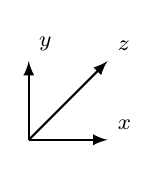
\begin{tikzpicture}
            \draw[ thick,-latex] (0,0) -- (1,0) node[anchor=south west] {$x$};
            \draw[ thick,-latex] (0,0) -- (0,1) node[anchor=south west] {$y$};
            \draw[ thick,-latex] (0,0) -- (1,1) node[anchor=south west] {$z$};
           \tkzText[above](-0.3,-0.7){}
        \end{tikzpicture} 
        \vspace{1cm}
        \fbox{\begin{tabular}{ll}
            \textcolor{fhrblue}{$\blacksquare$} & \gls{FLiBe} \\
            \textcolor{fhrgrey}{$\blacksquare$} & Graphite (Structure)\\
            \textcolor{fhrred}{$\blacksquare$} & Graphite (fuel plank) \\
            \textcolor{fhrblack}{$\blacksquare$} & TRISO particle 
            \end{tabular}}
    \end{subfigure}
    \caption{\acrfull{AHTR} one-third assembly geometry with a constant 0.0979 total packing 
    fraction across all fuel cells used for \gls{AHTR} one-third assembly's key neutronics 
    parameters verification. 
    The white line corresponds to the centerline where flux distribution is measured. }  
    \label{fig:ahtr-assem-verification}
\end{figure}

\subsubsection{AHTR One-Third Assembly: Effective Multiplication Factor}
Comparing $k_{eff}$ and reactivity produced by Moltres and OpenMC verify that the 
Moltres model replicates the OpenMC model's neutronics correctly.
Table \ref{tab:keff_ahtr_moltres_assem} compares the effective multiplication factor 
for OpenMC simulation with continuous energy and TRISO-level spatial fidelity, 
OpenMC simulation with 4-group energy and spatial homogenization, 
and Moltres simulation with 4-group energy and spatial homogenization.
I included results from a homogenized OpenMC simulation to 
distinguish between differences caused by spatial homogenization and energy 
discretization, or differing OpenMC and Moltres solve methods. 
\begin{table}[htbp]
    \centering
    \onehalfspacing
    \caption{\acrfull{AHTR} one-third assembly's $k_{eff}$ values from the OpenMC 
    simulation with continuous energy and TRISO-level spatial fidelity, 
    OpenMC simulation with 4-group energy and spatial homogenization, and Moltres 
    simulation with 4-group energy and spatial homogenization. 
    All simulations are at 948K.
    The normalized difference is the pcm difference normalized by OpenMC non-homogenized 
    model's $k_{eff}$.}
	\label{tab:keff_ahtr_moltres_assem}
    \footnotesize
    \begin{tabular}{lllclc}
        \hline 
        \textbf{Software}& \textbf{Homogenized?}& \textbf{$k_{eff}$} & \textbf{Diff [pcm]}  
        & \textbf{Reactivity [pcm]} & \textbf{Reactivity Diff [pcm]} \\
    \hline 
    OpenMC & No & $1.41657 \pm 0.00131$ & - & $29406 \pm 65$ & -\\ 
    OpenMC & Yes & $ 1.41670 \pm 0.00116$ & \Plus13 & $29413 \pm 58$& \Plus 7\\ 
    Moltres & Yes & $1.40895 $ & \Minus762 & 29025 & \Minus381 \\ 
    \hline
    \end{tabular}
\end{table} 

The 13pcm $k_{eff}$ and 7pcm reactivity difference between continuous and homogenized 
OpenMC simulations is within uncertainty, showing that the selected spatial 
homogenizationsand energy discretizations are acceptable. 
However, the Moltres simulation shows a $762pcm$ difference in $k_{eff}$ and 
$381pcm$ difference in reactivity, similar to the \gls{AHTR} plank model's difference 
in Section \ref{sec:plank-knp}.
The summary at the end of this section explains the differences in these values. 

\subsubsection{AHTR One-Third Assembly: Reactivity Coefficients}
A comparison of reactivity coefficients produced by Moltres and OpenMC verifies that 
the Moltres model is replicating the OpenMC model's neutronics correctly and are also 
important to ensure that Moltres accurately calculates the temperature distribution.
Moltres' delayed neutron fraction, $\beta{eff}$, is calculated by taking the 
normalized difference between $k_{eff}$ values with and without \glspl{DNP}. 
The $\beta{eff}$ values from OpenMC and Moltres in Table 
\ref{tab:ahtr_assem_moltres_coeffs} show excellent agreement with a discrepancy of
0.8pcm. 
I calculated the temperature reactivity coefficients with Equation 
\ref{eq:reactivity-coefficient}.
Table \ref{tab:ahtr_assem_moltres_coeffs} shows that the total temperature 
coefficients from OpenMC and Moltres have good agreement with a discrepancy of 
0.2 pcm/K.
\begin{table}[htbp]
    \centering
    \onehalfspacing
    \caption{\acrfull{AHTR} one-third assembly's $\beta_{eff}$ values from OpenMC and Moltres at 948K, and 
    total reactivity coefficient values calculated from OpenMC and Moltres at 948K and 1100K, 
    respectively.
    The OpenMC simulation has continuous energy and TRISO-level spatial fidelity.
    The Moltres simulation has 4-group energy and spatial homogenization.}
	\label{tab:ahtr_assem_moltres_coeffs}
    \footnotesize
    \begin{tabular}{llllll}
    \hline 
    \textbf{Software}& \textbf{Homogenized?}& \textbf{$\beta_{eff}$ [pcm]} 
    & \textbf{Diff [pcm]} & \textbf{Total $\frac{\Delta \rho}{\Delta T}$ [$pcm \cdot K^{-1}$]} 
    & \textbf{Diff [$pcm \cdot K^{-1}$]} \\
    \hline 
    OpenMC & No &  652.3 & - &  \Minus3.64 & - \\ 
    Moltres & Yes & 651.5 & \Minus0.8 & \Minus3.44 & \Plus0.2\\ 
    \hline
    \end{tabular}
\end{table}

\subsubsection{AHTR One-Third Assembly: Flux Distribution}
A comparison of flux distributions produced by Moltres and OpenMC verifies that the 
Moltres model is replicating the OpenMC model's neutronics correctly and are also 
important to ensure that Moltres accurately calculates the temperature distribution.
Figure \ref{fig:flux_948K_assem} shows the 4-group flux distributions for OpenMC and 
Moltres on the \gls{AHTR} one-third assembly's centerline, along the y-axis at 
the x-axis' midpoint (white line on Figure \ref{fig:ahtr-assem-verification}). 
\begin{figure}[htbp]
    \centering
    \includegraphics[width=0.48\linewidth]{flux_group1_948K_assem.png} 
    \includegraphics[width=0.48\linewidth]{flux_group2_948K_assem.png} 
    \includegraphics[width=0.48\linewidth]{flux_group3_948K_assem.png} 
    \includegraphics[width=0.48\linewidth]{flux_group4_948K_assem.png} 
    \caption{\acrfull{AHTR} one-third assembly's centerline neutron flux distribution 
    in 4 groups at 948K. 
    Centerline is the white line in Figure \ref{fig:ahtr-assem-verification}.
    The comparison is between the OpenMC simulation with continuous energy 
    and TRISO-level spatial fidelity and the Moltres simulation with 4-group energy and 
    spatial homogenization.
    Energy Group 1: E $> 9.1188 \times 10^{-3}$ MeV, 
    Energy Group 2: $2.9023 \times 10^{-5} < E < 9.1188 \times 10^{-3}$ MeV,
    Energy Group 3:  $1.8556 \times 10^{-5} < E < 2.9023 \times 10^{-5}$ MeV,
    Energy Group 4:  $1.0 \times 10^{-12} < E < 1.8554 \times 10^{-6}$ MeV.}
    \label{fig:flux_948K_assem}
\end{figure}
Table \ref{tab:ahtr-assem-verification-flux} reports the 2-norm percentage difference 
(Equation \ref{eq:ahtr-plank-flux-2norm}) and maximum percentage difference between 
centerline flux values from OpenMC and Moltres models. 
\begin{table}[htbp]
    \centering
    \onehalfspacing
    \caption{\acrfull{AHTR} one-third assembly's centerline 2-norm 
    flux percentage difference and maximum flux percentage difference. 
    Centerline is the white line in Figure \ref{fig:ahtr-assem-verification}.
    The difference values are calculated from comparison between the OpenMC simulation with 
    continuous energy and TRISO-level spatial fidelity and the Moltres simulation with 4-group energy 
    and spatial homogenization.}
	\label{tab:ahtr-assem-verification-flux}
    \footnotesize
    \begin{tabular}{lll}
    \hline 
    \textbf{Energy Group}& \textbf{2-norm Diff [$\%$]}& \textbf{Max Diff [$\%$]} \\
    \hline 
    1 & 0.15 & \Minus5.36 \\
    2 & 0.29 & \Plus7.13 \\
    3 & 0.33 & \Plus11.66 \\
    4 & 0.26 & \Plus5.82 \\
    \hline
    \end{tabular}
\end{table}

Figure \ref{fig:flux_948K_assem} shows that the OpenMC model has 
lower flux in Group 2 and 4 compared to the Moltres model. 
Table \ref{tab:ahtr-plank-verification-flux} shows that the 2-norm percentage differences 
between OpenMC and Moltres models' flux values are slight, demonstrating that there is a 
good overall agreement for each group's flux.
The summary at the end of this section explains the differences in the flux's maximum 
percentage differences between the OpenMC and Moltres models. 

\subsubsection{AHTR One-Third Assembly: Neutron Energy Spectrum}
A comparison of the neutron energy spectrum verifies that the Moltres model is replicating 
the OpenMC model's neutronics correctly.
Figure \ref{fig:assem_neutron_spectrum_948K} shows the one-third assembly's neutron 
spectrum of the OpenMC simulation for 252 and 4 groups and 4-group Moltres 
simulation. 
 \begin{figure}[htbp]
    \centering
    \includegraphics[width=\linewidth]{assem_neutron_spectrum_948K.png}
    \caption{\acrfull{AHTR} one-third assembly's neutron spectrum.
    Spectrums include 252 and 4 group spectrums from OpenMC simulation with continuous 
    energy and TRISO-level spatial fidelity and 4 group spectrum from Moltres 
    simulation with 4-group energy and spatial homogenization.}  
    \label{fig:assem_neutron_spectrum_948K}
\end{figure}
There is good agreement between OpenMC and Moltres models' 4-group spectrums. 

\subsubsection{AHTR One-Third Assembly: Key Neutronics Parameters Verification Summary}
The one-third assembly verification study has similar results to the plank verification 
study (Section \ref{sec:plank-knp}).
The verification study found a 381 pcm reactivity difference between OpenMC 
and Moltres models and good agreement in their reactivity coefficients and 4-group 
neutron energy spectrum.
The verification study also found good agreement in overall flux distributions 
(based on the 2-norm difference); however, there were larger flux differences at 
specific points. 
The reactivity and flux differences are due to Moltres utilizing the neutron diffusion 
method instead of neutron transport methods, resulting in flux not being reproduced 
well in small regions which are less than a few mean free paths in length 
(i.e., the FLiBe coolant channel). 
The differences in reactivity and flux at specific points might result in a slightly 
inaccurate absolute temperature distribution.  
However, since the reactivity coefficients and overall flux distribution are in 
agreement, Moltres accurately captures the relative temperature distributions. 
During the \gls{AHTR} optimization, so long the relative maximum temperature between 
different \gls{AHTR} models is captured correctly, \gls{ROLLO} can find optimal reactor 
geometries accurately. 
Reactor designers can then use higher fidelity software for modeling the final optimal 
\gls{AHTR} geometry. 
In summary, Moltres replicated the relevant neutronics parameters with sufficient 
accuracy using OpenMC's group constant data for the \gls{AHTR} one-third assembly model. 

\subsection{AHTR Plank and One-Third Assembly: Mesh Refinement Studies}
I performed mesh refinement studies on the \gls{AHTR} plank and one-third assembly 
Moltres temperature models to ensure that their geometry mesh inputs are sufficiently 
converged. 
Tables \ref{tab:ahtr-plank-mesh-refinement} and \ref{tab:ahtr-assem-mesh-refinement}
show the mesh refinement study results for the \gls{AHTR} plank and one-third 
assembly.
The mesh refinement studies report the average, maximum, and normalized 2-norm 
temperature difference between refinement steps. 
The 2-norm calculation is defined by Equation \ref{eq:2-norm-tdiff-i}. 
\begin{align}
    \label{eq:2-norm-tdiff-i}
    ||\Delta T_k||_N &= \frac{1}{N}\sqrt{\sum_{i=1}^N(T_{k-1, i} - T_{k, i})^2 }\\
\intertext{where}
    ||\Delta T_k||_N &= \mbox{normalized 2-norm temperature difference between refinement steps } [K] \nonumber \\
    N &= \mbox{total number of discretized points } [\#] \nonumber \\
    i &= \mbox{discretized point } [-] \nonumber \\
    k &= \mbox{refinement step } [-] \nonumber \\
    T_{k-1} &= \mbox{temperatures from previous refinement step } [K]\nonumber \\
    T_k &= \mbox{temperatures from current refinement step } [K]\nonumber 
\end{align} 
I used 100 discretized points (N) to calculate $||\Delta T_k||_N$ for all refinement 
steps.
\begin{table}[htbp]
    \centering
    \onehalfspacing
    \caption{\acrfull{AHTR} plank's Moltres temperature model mesh refinement study.}
	\label{tab:ahtr-plank-mesh-refinement}
    \scriptsize
    \begin{tabular}{lp{3.2cm}lp{3.2cm}ll}
        \hline 
        \textbf{Refinement} & \textbf{Max Plank Temp [K]} 
        & \textbf{Diff [K]} & \textbf{Avg Plank Temp [K]}
        & \textbf{Diff [K]} & $||\Delta T_k||_N$ [K]\\ 
        \hline 
        1 & 1126.219 & - & 1011.209 & - & - \\
        2 & 1127.711 & \Plus1.492 & 1017.630 & \Plus6.421 & 0.839\\
        3 & 1128.434 & \Plus0.723 & 1020.021 & \Plus2.390 & 0.313\\ 
        \hline
    \end{tabular}
\end{table}
\begin{table}[!tb]
    \centering
    \onehalfspacing
    \caption{\acrfull{AHTR} one-third assembly's Moltres temperature model mesh 
    refinement study.}
	\label{tab:ahtr-assem-mesh-refinement}
    \scriptsize
    \begin{tabular}{lp{3.2cm}lp{3.1cm}ll}
    \hline 
    \textbf{Refinement} & \textbf{Max One-Third Assembly Temp [K]} 
    & \textbf{Diff [K]} & \textbf{Avg One-Third Assembly Temp [K]}
    & \textbf{Diff [K]} & $||\Delta T_k||_N$ [K]\\ 
    \hline 
    1 & 1185.436 & - & 995.963 & - & - \\
    2 & 1186.045 & \Plus0.609 & 1001.751 & \Plus5.788 & 0.703\\
    3 & 1185.994 & \Minus0.051 & 1003.625 & \Plus1.874 & 0.200\\
    \hline
    \end{tabular}
\end{table}

For each Moltres temperature model, I must balance convergence and computational cost, 
thus, I determine that mesh convergence is met if $||\Delta T_k||_N < 0.5K$. 
Both \gls{AHTR} plank and one-third assembly show suitable $||\Delta T_k||_N$ 
convergence at x3 mesh refinement; thus I used x3 mesh refinement for all 
\gls{AHTR} plank and one-third assembly Moltres temperature models. 
Further refinement is computationally unfeasible due to the large mesh size. 
I used the Theta supercomputer \cite{noauthor_thetathetagpu_2022} for the 
optimization work.
Each supercomputer node saves the entire mesh file, further refinement results in 
mesh sizes that are larger than each Theta node's memory size. 

\subsection{AHTR Plank and One-Third Assembly: Group Constant Temperature Study}
During ROLLO optimization, each new reactor model results in the creation of 
a new Moltres temperature model. 
Correspondingly, a new set of group constant data needs to be created for each 
Moltres temperature model.
Moltres relies on the OpenMC model to generate group constant data for the 
Moltres' multigroup neutron diffusion calculations. 
The Moltres model uses the group constant data by interpolating it for its 
required temperatures.
Group constant data with multiple temperatures requires running multiple OpenMC 
neutronics simulations at the various temperatures, thus, increasing the total 
compute time required for each new reactor model. 
This section explores the effects of using multiple temperature group 
constant data compared to single temperature group constant data.
I set up Moltres \gls{AHTR} steady-state temperature models for the plank and one-third 
assembly with group constant data at each and all the of following temperatures: 948, 
1024, 1100, and 1200K. 

Tables \ref{tab:moltres-group-constant-temps} and 
\ref{tab:moltres-group-constant-temps-assem}
show the average and maximum temperature reported by the \gls{AHTR} plank and one-third 
assembly Moltres models using group constant data from one temperature and their 
differences compared to the model with group constant data with all four temperatures. 
Both tables also show the normalized 2-norm of the centerline temperature difference 
between the \gls{AHTR} models with single temperatures and the \gls{AHTR} model with all four 
temperature (Equation \ref{eq:2-norm-tdiff-all}):
\begin{align}
    \label{eq:2-norm-tdiff-all}
    ||\Delta T||_N &= \frac{1}{N}\sqrt{\sum_{i=1}^N(T_{all, i} - T_{i})^2} \\
\intertext{where}
    ||\Delta T||_N &= \mbox{normalized 2-norm temperature difference } [K]\nonumber \\
    N &= \mbox{total number of discretized points } [\#] \nonumber \\
    i &= \mbox{discretized point } [-] \nonumber \\
    T_{all} &= \mbox{temperatures from model with group constant data at all four temperatures } [K] \nonumber \\
    T &= \mbox{temperatures from model with group constant data at one temperature } [K] \nonumber 
\end{align}
The centerlines where the temperature (T) is measured in the model for the \gls{AHTR} 
plank and one-third models are depicted in Figures \ref{fig:ahtr-plank-verification} 
and \ref{fig:ahtr-assem-verification}, respectively. 

\begin{table}[htbp]
    \centering
    \onehalfspacing
    \caption{\acrfull{AHTR} plank's average and maximum temperature and normalized 
    2-norm of the temperature difference across the plank's centerline for 
    varying group constant temperature data. The difference values are calculated from 
    comparison against the Moltres model using group constant data with all four 
    temperatures (All).}
	\label{tab:moltres-group-constant-temps}
    \scriptsize
    \begin{tabular}{p{2.5cm}p{2cm}p{2.4cm}p{2cm}p{2.4cm}p{2cm}}
    \hline 
    \textbf{Group Constant Data Temps [K]}& \textbf{Avg Plank Temp [K]}& 
    \textbf{Avg Plank Temp Diff [K]}& \textbf{Max Plank Temp [K]} & 
    \textbf{Max Plank Temp Diff [K]} & $||\Delta T||_N$ \\ 
    \hline 
    All  & 1019.965 &  -     & 1128.306 & -      & -    \\
    948  & 1019.997 &  \Plus0.032 & 1128.386 & \Plus0.080 & 0.007\\
    1024 & 1019.989 &  \Plus0.023 & 1128.640 & \Plus0.333 & 0.023 \\
    1100 & 1019.976 &  \Plus0.011 & 1128.300 & \Minus0.006 & 0.029 \\
    1200 & 1019.943 & \Minus0.023 & 1128.052 & \Minus0.255 & 0.043 \\
    \hline
    \end{tabular}
\end{table}
The temperature differences between the \gls{AHTR} plank model using group constants at 
all four temperatures and the \gls{AHTR} plank models' using group constants at each 
single temperature are not significant. 
Since all the single temperature group constant data in Table 
\ref{tab:moltres-group-constant-temps} have non-significant temperature differences, 
any of them could be used for the Moltres temperature models.
The 948K single temperature group constant data has the lowest 2-norm difference 
($||\Delta T||_N$). 
Thus, I chose to use a 948K in the \gls{AHTR} plank OpenMC neutronics model to 
generate the group constant data for the Moltres temperature models.

\begin{table}[htbp]
    \centering
    \onehalfspacing
    \caption{\acrfull{AHTR} one-third assembly's average and maximum temperature and 
    2-norm of the temperature difference across the slab's centerline for varying 
    group constant temperature data. The difference values are calculated from 
    comparison against the Moltres model using group constant data with all four 
    temperatures (All).}
	\label{tab:moltres-group-constant-temps-assem}
    \scriptsize
    \begin{tabular}{p{2.5cm}p{2.5cm}p{2cm}p{2.5cm}p{2cm}p{2cm}}
    \hline 
    \textbf{Group Constant Data Temps [K]}& \textbf{Avg One-Third Assembly Temp [K]}& 
    \textbf{Diff [K]}& \textbf{Max One-Third Assembly Temp [K]} & 
    \textbf{Diff [K]} & $||\Delta T||_N$ \\ 
    \hline 
    All  & 1004.366 &  -     & 1186.359 & -      & -    \\
    948  & 1004.708 & \Plus0.341 & 1187.658 & \Plus1.299 & 0.044 \\
    1024 & 1004.676 & \Plus0.310 & 1187.148 & \Plus0.788 & 0.041 \\
    1100 & 1004.622 & \Plus0.256 & 1186.085 & \Minus0.274 & 0.046\\
    1200 & 1004.539 & \Plus0.172 & 1185.359 & \Minus1.000 & 0.047 \\
    \hline
    \end{tabular}
\end{table}
The temperature differences between the \gls{AHTR} one-third assembly model using group 
constants at all four temperatures and the \gls{AHTR} plank models using group 
constants at a single temperature are small ($<1K$). 
The 1024K single temperature group constant data has the lowest 2-norm difference 
($||\Delta T||_N$). 
Thus, I use 1024K in the \gls{AHTR} one-third assembly OpenMC neutronics model to 
generate the group constant data for the Moltres temperature models.

\section{ROLLO Hyperparameter Tuning}
\label{sec:hyperparameter-studies}
Recall from Chapter \ref{chap:lit-review}, I discussed how genetic algorithms 
require a good hyperparameter set that guides the optimization process by 
balancing exploitation and exploration to find an optimal solution quickly 
and accurately \cite{deb_multi-objective_2001}. 
Finding a good hyperparameter set requires a trial-and-error process 
\cite{deb_multi-objective_2001}. 
In a \gls{ROLLO} input file, the user defines hyperparameters for the genetic 
algorithm.
The subsequent subsections describe the hyperparameter search I conducted for 
single-objective and multi-objective optimization. 

\subsection{ROLLO Single-Objective Optimization Hyperparameters}
\label{sec:rollo-single-hyp}
I performed the single-objective hyperparameter search with a coarse-to-fine random 
sampling scheme, whose advantages I previously discussed in Section \ref{sec:balance}.
I used an \gls{AHTR} plank OpenMC model for the hyperparameter search (Figure 
\ref{fig:straightened_plank}). 
The hyperparameters are population size, number of generations, 
mutation probability, mating probability, selection operator, selection operator's 
number of individuals, selection operator's tournament size, mutation operator, 
and mating operator.  
I started with 25 coarse experiments and fine-tuned the hyperparameters
with 15 more experiments. 
For each genetic algorithm experiment, total number of OpenMC models run 
remained constant at 600.
The number of evaluations correlates with the population size and the number of 
generations. 
I randomly sampled population size and used Equation \ref{eq:pop_gen} to calculate 
the number of generations: 
\begin{align}
    \label{eq:pop_gen}
    gens &= \frac{evals}{pop\_size} \\
         &= \frac{600}{pop\_size} \nonumber 
    \intertext{where}
    gens &= \mbox{no. of generations} \nonumber \\
    evals &= \mbox{no. of evaluations} \nonumber \\
    pop\_size &= \mbox{population size} \nonumber
\end{align}
Table \ref{tab:hyperparameter_search} shows the lower and upper bounds used 
for randomly sampling each hyperparameter at each phase of the hyperparameter search.
\begin{table}[htbp]
    \centering
    \onehalfspacing
    \caption{The hyperparameter search is conducted in three phases: \textit{Coarse Search}, 
    \textit{Fine Search 1}, \textit{Fine Search 2}. Each hyperparameter's lower and
    upper bounds for each search phase are listed.}
	\label{tab:hyperparameter_search}
    \footnotesize
    \makebox[\textwidth][c]{\begin{tabular}{p{4cm}lp{3.4cm}p{3.4cm}p{3.4cm}}
    \hline 
    \textbf{Hyperparameter}& \textbf{Type} & \textbf{Coarse Search Bounds} & \textbf{Fine Search 1 Bounds} & \textbf{Fine Search 2 Bounds} \\
    \hline
    Experiments [\#] & - & 0 to 24 & 24 to 34 & 35 to 39 \\ 
    \hline
    Population size [\#] & Continuous & 10 $<$ x $<$ 100 & 20 $<$ x $<$ 60 & 60 \\ 
    Mutation probability [-] & Continuous & 0.1 $<$ x $<$ 0.4 & 0.2 $<$ x $<$ 0.4& 0.2 $<$ x $<$ 0.3\\
    Mating probability [-] & Continuous & 0.1 $<$ x $<$ 0.6 &  0.1 $<$ x $<$ 0.3 &  0.45 $<$ x $<$ 0.6\\
    Selection operator [-] & Discrete & \texttt{SelTournament}, \texttt{SelBest}, \texttt{SelNSGA2} & \texttt{SelTournament}, \texttt{SelBest}, \texttt{SelNSGA2}& \texttt{SelTournament}\\
    Selection individuals [\#] & Continuous & $\frac{1}{3}pop$ $<$ x $<$ $\frac{2}{3}pop$ & $\frac{1}{3}pop$ $<$ x $<$ $\frac{2}{3}pop$ & 15\\
    Selection tournament size (only for SelTournament) [\#] & Continuous & 2 $<$ x $<$ 8 &2 $<$ x $<$ 8&5\\
    Mutation operator [-] & Discrete & \texttt{mutPolynomialBounded} &\texttt{mutPolynomialBounded}&\texttt{mutPolynomialBounded}\\
    Mating operator [-] & Discrete& \texttt{cxOnePoint}, \texttt{cxUniform}, \texttt{cxBlend} &\texttt{cxOnePoint}, \texttt{cxUniform}, \texttt{cxBlend}&\texttt{cxOnePoint}, \texttt{cxBlend}\\ 
    \hline
    \end{tabular}}
\end{table}

The initial 25 coarse experiments sought to narrow down the hyperparameters 
to find a smaller set of hyperparameter bounds that produce higher $k_{eff}$ values.
Figure \ref{fig:hyperparameter_sens} shows the hyperparameters plotted against 
each other with a third color dimension representing the average $k_{eff}$ value
($\overline{k_{eff}}$) in each experiment's final generation. 
Lighter scatter points indicate higher final population $\overline{k_{eff}}$ values, 
suggesting better hyperparameter sets. 
\begin{figure}[htbp]
    \centering
    \makebox[\textwidth][c]{\includegraphics[width=1.3\linewidth]{hyperparameter_sens.png}} 
    \caption{Coarse \acrfull{ROLLO} hyperparameters search's results. 
    Hyperparameter values are plot against each other with a third color dimension 
    representing each experiment's final population's $\overline{k_{eff}}$.}
    \label{fig:hyperparameter_sens}
\end{figure}
I plot the hyperparameters against each other to visualize the interdependence 
between hyperparameters. 
From the coarse hyperparameter search (Figure \ref{fig:hyperparameter_sens}), 
I noticed the following trends: 
\begin{itemize}
    \item Mutation probability has a higher $\overline{k_{eff}}$, between 0.2 and 0.4. 
    \item Mating probability has a higher $\overline{k_{eff}}$, between 0.1 and 0.3. 
    \item Population size has a higher $\overline{k_{eff}}$, between 20 and 60. 
    \item No obvious interdependence between hyperparameters. 
\end{itemize} 

Next, I proceeded to the fine searches. 
From Figure \ref{fig:hyperparameter_sens}, I narrowed down population size, 
mutation probability, and mating probability bounds, as shown in Table 
\ref{tab:hyperparameter_search}'s \textit{Fine Search 1 Bounds} column. 
I found no significant trends in the other hyperparameters, so I left them 
as is. 
I ran ten more experiments (25 to 34), sampling hyperparameters from 
the \textit{Fine Search 1 Bounds}. 
From these results, I conducted a second fine search with five experiments 
(35 to 39) with further tuned hyperparameter bounds, as shown in Table 
\ref{tab:hyperparameter_search}'s \textit{Fine Search 2 Bounds} column. 
I determined these new hyperparameter bounds based on these reasons: 
\begin{itemize}
    \item Mutation probability has a higher $\overline{k_{eff}}$, between 0.2 and 0.3.
    \item I overlooked $\overline{k_{eff}}$  peaking at mating probability between 
    0.45 and 0.6 in the previous \textit{Fine Search 1}; thus, I shifted the bounds. 
    \item The highest $\overline{k_{eff}}$ occurred for \texttt{selTournament}. 
    \item I narrowed down mating operator options to \texttt{cxBlend} and 
    \texttt{cxOnePoint} since they had higher $\overline{k_{eff}}$ than 
    \texttt{cxUniform}. 
    \item I selected arbitrary numbers for population size, 
    selection individuals, and tournament size since they did not 
    correlate with $\overline{k_{eff}}$ values. 
\end{itemize}
Figure \ref{fig:input_hyperparameters_sens} shows the relationship between 
hyperparameter values and $a$, $b$, $c$ control variables, final generation 
$k_{eff max}$, and final generation $\overline{k_{eff}}$. 
The coarse experiments' scatter points are $50\%$ transparent, while the fine 
experiments' scatter points are opaque. 
\begin{figure}[htbp]
    \centering
    \makebox[\textwidth][c]{\includegraphics[width=1.3\linewidth]{input_hyperparameters_sens.png}} 
    \caption{ \acrfull{ROLLO} hyperparameter search results for all 40 experiments 
    (coarse and fine). I plot the hyperparameters against: the \textit{a, b, c} control 
    variables, each experiment's final generation $k_{eff max}$, and the final generation 
    $\overline{k_{eff}}$ with a third color dimension representing each experiment's final 
    population's $\overline{k_{eff}}$ (color bar representing the $k_{eff}$ values 
    provided on the right side of the figure). Coarse experiments' (0 to 24) scatter points 
    are $50\%$ transparent, while the fine experiments' (24 to 39) scatter points 
    are opaque. }
    \label{fig:input_hyperparameters_sens}
\end{figure}
In Figure \ref{fig:input_hyperparameters_sens}, on average, the fine experiments 
(opaque scatter points) have higher $\overline{k_{eff}}$, which indicates that the
hyperparameter search process met its objective of finding hyperparameter 
bounds that enable quicker and more accurate optimization. 

I ran these hyperparameter search simulations on the BlueWaters supercomputer 
\cite{ncsa_about_2017}. 
In each \gls{ROLLO} simulation, each generation runs a population size number 
of individual OpenMC simulations. 
Each OpenMC simulation takes approximately 13 minutes to run on a single BlueWaters 
XE node. 
With approximately 600 OpenMC evaluations per \gls{ROLLO} simulation, one
\gls{ROLLO} simulation takes about 130 BlueWaters node-hours. 
The hyperparameter search ran 40 \gls{ROLLO} simulations, thus using approximately
5200 node-hours.

I define the best-performing hyperparameter set as the experiment that produces 
the highest $\overline{k_{eff}}$ in its final generation. 
Table \ref{tab:topfive} shows the hyperparameters for the five experiments 
with the highest final generation $\overline{k_{eff}}$.
\begin{table}[htbp]
    \centering
    \onehalfspacing
    \caption{Control variables, $k_{eff}$ results, and hyperparameter values for 
    the five hyperparameter search experiments with the highest final generation 
    $\overline{k_{eff}}$.}
	\label{tab:topfive}
    \scriptsize
    \makebox[\textwidth][c]{\begin{tabular}{p{3.2cm}p{2.6cm}p{2.6cm}p{2.6cm}p{2.6cm}p{2.6cm}}
    \hline 
    & \multicolumn{5}{c}{\textbf{Experiment No.}} \\
    \cline{2-6}
    \textbf{Control/Output Variables} & \textbf{6} & \textbf{15} & \textbf{24} & \textbf{36} & \textbf{39}\\
    \hline 
    $\overline{k_{eff}}$ [-] & 1.39876 &1.40155&1.40118&1.39906&1.40165\\ 
    $k_{eff max}$ [-] & 1.40954 &1.40440&1.40365&1.40590&1.40519\\ 
    a [-] & 1.993&1.998&1.999&1.997&1.989\\
    b [$radians \cdot cm^{-1}$] & 0.057&0.367&0.320&0.339&0.354\\ 
    c [$radians$] & 3.571&3.022&3.615&3.053&3.143\\
    \hline
    \textbf{Hyperparameter}& &&&&\\
    Population size [\#] & 83 & 28&74&60&60\\ 
    Generations [\#] &8&22&9&10&10 \\
    Mutation probability [-] & 0.32 &0.26&0.21&0.23&0.23\\
    Mating probability [-] & 0.17 &0.53&0.48&0.59&0.46\\
    Selection operator [-]& \texttt{selTournament} &\texttt{selTournament}&\texttt{selBest}&\texttt{selTournament}&\texttt{selTournament}\\
    Selection individuals [\#] & 38 &14&25&15&15\\
    Selection tournament size [\#] & 7 &5&-&5&5\\
    Mutation operator [-] & \texttt{mutPolynomial} \texttt{Bounded}&\texttt{mutPolynomial} \texttt{Bounded}&\texttt{mutPolynomial} \texttt{Bounded}&\texttt{mutPolynomial} \texttt{Bounded}&\texttt{mutPolynomial} \texttt{Bounded}\\
    Mating operator [-] & \texttt{cxOnePoint} &\texttt{cxOnePoint}&\texttt{cxUniform}&\texttt{cxBlend}&\texttt{cxBlend}\\ 
    \hline
    \end{tabular}}
\end{table}
\textit{Fine Search 2}'s experiment 39 produces the best performing 
hyperparameter set, with $\overline{k_{eff}} = 1.40165ß$. 
Therefore, for single-objective ROLLO optimization simulations in this dissertation, 
I use the hyperparameter set from experiment 39. 

\subsection{ROLLO Multi-Objective Optimization Hyperparameters}
\label{sec:multi-obj-hyperparameters}
Due to a lack of computational resources, I did not use an OpenMC example problem or 
a coarse-to-fine random sampling scheme for the multi-objective optimization 
hyperparameter search.
I used the Binh and Korn function described in Section \ref{sec:binhandkorn} as 
an example problem to conduct the hyperparameter search.

I conducted a simpler hyperparameter search for the multi-objective optimization case. 
I chose to use \texttt{SelNSGA2} for the selection operator, since it is an elitist 
operator that works well for multi-objective optimization. 
Next, I varied each of the following parameters individually and compared their 
hypervolume values: population size/generations, mutation probability, and mating 
probability.
Section \ref{sec:binhandkorn} described that the hypervolume indicator quantifies 
how well the multi-objective optimization's Pareto front covers the 
multi-objective domain (bigger = better). 

Figure \ref{fig:hypervolume-comparison} shows boxplots comparing hypervolumes 
for various hyperparameters. 
I ran each simulation 25 times to produce each box plot. 
\begin{figure}[htbp]
    \centering
    \begin{subfigure}{0.55\textwidth}
    \makebox[\textwidth][c]{\includegraphics[width=\linewidth]{hypervolume-comparison-gens.png}} 
    \caption{Population size / Generation variation.}
    \label{fig:hypervolume-comparison-gens}
    \end{subfigure}
    \begin{subfigure}{0.55\textwidth}
        \makebox[\textwidth][c]{\includegraphics[width=\linewidth]{hypervolume-comparison-matpb.png}}
        \caption{Mating probability variation}
        \label{fig:hypervolume-comparison-matpb}
    \end{subfigure}
    \begin{subfigure}{0.55\textwidth}
        \makebox[\textwidth][c]{\includegraphics[width=\linewidth]{hypervolume-comparison-mutpb.png}}
        \caption{Mutation probability variation}
        \label{fig:hypervolume-comparison-mutpb}
    \end{subfigure}
    \caption{Hypervolume comparisons for varying \acrfull{ROLLO} hyperparameters for the
    multi-objective optimization hyperparameter search. }
    \label{fig:hypervolume-comparison}
\end{figure}
Figure \ref{fig:hypervolume-comparison-gens} shows the boxplot comparing hypervolume 
for different population size and generation combinations. 
Similar to Section \ref{sec:rollo-single-hyp}, I held the total number of OpenMC 
evaluations constant at 600. 
Equation \ref{eq:pop_gen} shows the relationship between population size and generations. 
The combination of 120 population size and 5 generations performs the best with the 
highest hypervolume median (orange line). 

Figure \ref{fig:hypervolume-comparison-matpb} shows a boxplot comparing hypervolume 
for different mating probabilities. 
The 0.9 mutation probability performs the best with the highest hypervolume median 
(orange line), compared to the 0.46 from the best single-objective hyperparameter set 
(Section \ref{sec:rollo-single-hyp}). 
Figure \ref{fig:hypervolume-comparison-mutpb} shows a boxplot comparing hypervolume 
for different mutation probabilities. 
The 0.23 mating probability from the best single-objective hyperparameter set 
(Section \ref{sec:rollo-single-hyp}) performs as well as the 0.1 mating probability. 

Based on the box plot comparisons, I selected the combination of hyperparameters that 
maximized the hypervolume. 
Table \ref{tab:multi-obj-hyp} summarizes the hyperparameters I used for \gls{ROLLO} 
multi-objective optimization.  
\begin{table}[htbp]
    \centering
    \onehalfspacing
    \caption{\acrfull{ROLLO} hyperparameters used for multi-objective optimization.}
	\label{tab:multi-obj-hyp}
    \footnotesize
    \begin{tabular}{ll}
    \hline 
    \textbf{Hyperparameter} & \textbf{Value} \\
    \hline 
    Population size & 120 \\
    Generations & 5 \\
    Mutation probability & 0.9 \\
    Mating probability & 0.23 \\
    Selection operator & \texttt{SelNSGA2} \\
    Mutation operator & \texttt{mutPolynomial} \texttt{Bounded} \\
    Mating operator & \texttt{cxBlend} \\
    \hline
    \end{tabular}
\end{table}
Reactor designers with ample computational power may use a reactor 
modeling problem to conduct their multi-objective optimization hyperparameter search. 
Using hyperparameters optimized for their reactor model could reduce the number of 
generations required to find a Pareto front with a large hypervolume and also enable 
finding a more optimal Pareto front.  
However, using the multi-objective hyperparameters outlined in Table 
\ref{tab:multi-obj-hyp} is sufficient for any reactor designers that do not want to 
conduct a problem-specific hyperparameter search. 

\section{Summary}
\glsresetall
This chapter describes the modeling and optimization methodology of the 
\gls{AHTR} plank and one-third assembly optimization for non-conventional 
geometries and parameters conducted using the \gls{ROLLO} software.
I defined and described the \gls{AHTR} input parameters varied for the optimization 
problems. 
The input parameters include \gls{TRISO} packing distribution, total fuel packing 
fraction, and coolant channel shape. 
I defined and motivated the key optimization objectives: minimizing fuel amount,
maximizing heat transfer, and minimizing power peaking (Table \ref{tab:objectives}).
I described the \gls{AHTR} plank and one-third assembly geometries and  
detailed their modeling workflow: the \gls{AHTR} input parameter variations, 
the OpenMC neutronics model, the Moltres temperature model, and 
the output constraint and objective value calculations. 
I conducted key neutronics parameter verifications, which confirmed that the spatial 
and energy homogenizations used for the \gls{AHTR} plank and one-third assembly Moltres 
temperature models preserved accuracy.
Finally, I described the \gls{ROLLO} hyperparameter tuning process and reported the 
hyperparameters used for the single and multi-objective optimization problems. 

Chapters \ref{chap:ahtr-plank-opt-results} and \ref{chap:ahtr-assem-opt-results} 
report the \gls{AHTR} plank and \gls{AHTR} one-third assembly optimization results 
that use this chapter's described methods.